
\chapter{Mengen, Relationen und Funktionen}

Die Mengenlehre stellt einen formalen Rahmen zur Verfügung, der es erlaubt, mehrere mathematische Objekte
zusammenzufassen und diese Zusammenfassung als neues eigenständiges Objekt zu verstehen. Der Prozess der Mengenbildung und das Konzept einer Menge sind fundamental für den gesamten Aufbau der Mathematik aber nicht immer unproblematisch. Die Probleme, die ein allzu naiver Umgang mit Mengenexistenzannahmen verursachen können, zeigen sich zum Beispiel in der ``Russelschen Antinomie''. Die Russelsche Antinomie verdeutlicht, dass man nicht beliebige Dinge anhand einer Eigenschaft zu einer Menge zusammenfassen kann. Das Paradox entsteht, wenn man naiverweise davon ausgeht, dass zu jeder Eigenschaft $\mathsf{E}$ die Menge aller Dinge mit der Eigenschaft $\mathsf{E}$
\[
\{x\mid x\text{ hat die Eigenschaft } \mathsf{E}(x)\}
\]
 gebildet werden kann. Ein solches Prinzip lässt die Bildung der paradoxen Menge
 \[
 R=\{x\mid x\notin x\}
 \]
aller Mengen, die sich nicht selbst als Element enthalten, zu. Die Menge $R$ ist widersprüchlich, weil sowohl $R\in R$ als auch $R\notin R$ im Widerspruch zur definierenden Eigenschaft von $R$ steht.

In diesem Kapitel untersuchen wir, wie sich ein adäquater Umgang mit Mengen und Mengenbildung ausgestalten lässt. Weiter werden wir am Beispiel von Relationen und Funktionen sehen, dass Mengen ein mächtiges Werkzeug darstellen, das dazu geeignet ist, alle möglichen mathematischen Konstrukte präzise zu beschreiben.


\section*{Relevanz für die Informatik}
Die Bedeutung der Mengenlehre für die Informatik kommt weniger von direkten Anwendungen, sondern von ihrer Stellung innerhalb der Mathematik - Mengen sind in gewisser Weise der \textit{primitive Datentyp} der (modernen) Mathematik. Dies hat unter anderem folgende Konsequenzen:
\begin{itemize}
\item Die Mengenlehre bildet (zusammen mit der Prädikatenlogik) die Sprache der Mathematik.
\item Alle mathematischen Objekte sind Mengen, insbesondere sind auch alle in der theoretischen Informatik behandelten Strukturen (berechenbare Funktionen, Turing Maschinen, \dots) Mengen.
\end{itemize}
Weitere in diesem Kapitel behandelte Konzepte wie Funktionen und Relationen sind sowohl in der Mathematik als auch in der Informatik nahezu allgegenwärtig:
\begin{itemize}
\item Funktionen in der (funktionalen) Programmierung
\item Input-Output Relation
\item Relationale Datenbanken
\item E-R-Diagramme
\item Zustandsklassen von endlichen Automaten
\item $\vdots$
\end{itemize}
Graphen und (binäre) Relationen sind im wesentlichen gleichwertig, in der Tat können
Graphen auf natürliche Art und Weise dazu verwendet werden, Relationen grafisch
darzustellen. In der Informatik sind Graphen (insbesondere Bäume) eine der
fundamentalen Datenstrukturen (eine Art Daten zu organisieren).



\section*{Lernziele}
Sie kennen
\begin{itemize}
\item die grundlegenden mengentheoretischen Operationen (Vereinigung, Schnitt, Komplement, Potenzmenge).
\item die Zahlenmengen $\N,\Z,\Q$ und $\R$.
\item die verschiedenen Darstellungsformen für Mengen.
\item den Funktionsbegriff.
\item Äquivalenzrelationen und Äquivalenzklassen sowie ihre grundlegenden Eigenschaften.
\item Ordnungsrelationen (in den verschiedenen Variationen) und ihre grundlegenden
Eigenschaften.
\item grundlegende Typen von Graphen.
\end{itemize}
Sie verstehen
\begin{itemize}
\item den Zusammenhang von Funktionen, Relationen und Graphen.
\item den Zusammenhang von Äquivalenzrelationen und Partitionen.
\item die Problematik der ``Wohldefiniertheit'' von Funktionen auf Faktormengen.
\item wie man Relationen mit Graphen darstellen kann.
\item wie man Mengen in ihrer Mächtigkeit vergleicht.
\item den Unterschied zwischen einer abzählbaren und einer überabzählbaren Menge.
\end{itemize}
Sie sind in der Lage
\begin{itemize}
\item (endliche) Ordnungsrelationen als Hasse Diagramme zu skizzieren.
\item eine Ordnungsrelation aus einem Hasse Diagramm abzulesen.
\item Argumente für die Abzählbarkeit von $\Z$, $\Q$ und ähnlichen Mengen anzugeben.
\item zu beweisen, dass $\R$ und ähnliche Mengen überabzählbar sind.
\end{itemize}


\section*{Literatur und Links}
Ergänzende Literatur:
\begin{itemize}
\item \cite{diskreteStrukturen} Kapitel 2 ohne 2.4 und 2.5.
\item \cite{diskreteStrukturen} Kapitel 4.1 bis 4.3.
\item \cite{pareigis} Kapitel 1 Teil 1 und Kapitel 1.4 sowie 1.5.
\end{itemize}
Nützliche Links:
\begin{itemize}
\item \url{http://de.wikipedia.org/wiki/Menge_(Mathematik)}
\item \url{http://builds.openlogicproject.org/courses/set-theory/settheory-screen.pdf} Kapitel 2. und 5.
\item \url{http://de.wikipedia.org/wiki/Relation_%28Mathematik%29}
\item \url{https://de.wikipedia.org/wiki/Graph_(Graphentheorie)}
\end{itemize}


\section{Der Mengenbegriff und grundlegende Definitionen}

Wenn jedes mathematische Objekt eine Menge ist, was ist dann die mathematische Definition einer Menge? Dies ist in der Tat nicht ganz einfach und wird in der Literatur meist auf eine der folgenden Arten behandelt:
\begin{itemize}
\item Einführung einer formalen Axiomatisierung der (oder einer) Mengenlehre.
\item Auf eine Definition wird verzichtet, stattdessen werden wichtige ``definierende'' Eigenschaften von Mengen festgehalten. Dieser Ansatz entspricht von der Idee her dem ersten Ansatz, ist aber weniger formal ausgelegt.
\item Eine anschauliche ``Definition'' zu verwenden, die zwar den Standards einer mathematischen Definition nicht genügt, aus der sich aber trotzdem wichtige Eigenschaften von Mengen anschaulich ableiten lassen.
\end{itemize}
Wir wählen die zweite Variante und bauen unseren Mengenbegriff dadurch auf, dass wir einige \textit{definierende} \textit{Eigenschaften} und Schreibweisen für Mengen einführen.

Die wichtigste Schreibweise im Umgang mit Mengen ist die Notation, die ausdrückt, ob etwas zu einer Menge gehört oder nicht.

\begin{nt}
Ist $X$ eine Menge und $y$ ein \textit{Element} von $X$, dann schreiben wir $y\in X$. Ist $y$ kein Element von $X$, dann schreiben wir $y\notin X$.
\end{nt}

Die erste \textit{definierende Eigenschaft} von Mengen ist die Tatsache, dass jede Menge durch ihre Elemente vollständig beschrieben ist.

\begin{df}[Definierende Eigenschaft]
Zwei Mengen sind genau dann gleich, wenn sie dieselben Elemente enthalten: Es gilt für alle Mengen $X$ und $Y$ die Äquivalenz
\[
X=Y\,\Leftrightarrow\,\forall z\, (z\in X\Leftrightarrow z\in Y).
\]
\end{df}

Da Mengen bereits durch Angabe ihrer Elemente bestimmt werden, können wir jede (endliche) Menge durch Auflisten ihrer Elemente festlegen.

\begin{df}[Explizite Schreibweise]
Sind mathematische Objekte $x_1,\dots,x_n$ gegeben, dann schreiben wir
\[
\{x_1,\dots,x_n\}
\]
für die Menge die als Elemente genau $x_1,\dots,x_n$ hat.
\end{df}

\begin{bsp}~
\begin{itemize}
\item Die Menge $\{2,34,77\}$ enthält die drei Elemente $2$, $34$ und $77$.
\item Die Menge $\{\,\}$ heisst \textit{leere Menge}. Die leere Menge ist die einzige Menge, die gar keine Elemente besitzt, sie wird mit $\varnothing $ bezeichnet.
\end{itemize}
\end{bsp}

\begin{rk}
Wenn keine Missverständnisse zu befürchten sind, so beschreibt man Mengen auch durch ``angedeutete'' Aufzählung ihrer Elemente. Die Menge $\mathbb{N}$ der \textit{natürlichen Zahlen} wird beispielsweise durch
\[
\N:=\{0,1,2,\dots\}
\]
beschrieben. Die Menge der \textit{ganzen Zahlen} wird durch
\[
\Z:=\{\dots, -2,-1,0,1,2\dots\}
\]
beschrieben.
\end{rk}

\begin{rk}
Die Tatsache, dass Mengen durch ihre Elemente eindeutig beschrieben werden hat zur Folge, dass Mengen sehr ``unstrukturierte Datentypen'' sind, d.h. Mengen haben keine ``innere Ordnung''. Es gelten unter anderem:
\begin{itemize}
\item Für beliebige $z,x_1,\dots,x_n$
\[
z\in\{x_1,\dots x_n\}\,\Leftrightarrow\, z=x_1\lor\dots\lor z=x_n
\]
\item Für alle $x$
\[
\{x\}=\{x,x\}=\{x,x,x\}=\dots
\]
\item Für alle $x,y$
\[
\{x,y\}=\{y,x\}.
\]
\end{itemize}
\end{rk}

\begin{df}[Teilmengen]
 Wir schreiben $X\subseteq Y$ und sagen $X$ ist eine \textit{Teilmenge} von $Y$, wenn jedes Element von $X$ auch ein Element von $Y$ ist:
\[
X\subseteq Y:\,\Leftrightarrow\,\forall x\,(x\in X\Rightarrow x\in Y).
\]
Wir schreiben $X\subsetneq Y$ und sagen $X$ ist eine \textit{echte Teilmenge} von $Y$, falls $X$ eine von $Y$ verschiedene Teilmenge von $Y$ ist:
\[
X\subsetneq Y\,:\Leftrightarrow\, X\subseteq Y\land X\neq Y.
\]
\end{df}

\begin{bsp}~
\begin{itemize}
\item Die Menge aller Hühner ist eine (echte) Teilmenge der Menge aller Vögel, weil alle Hühner Vögel sind (und weil es Vögel gibt die keine Hühner sind).
\item Die Menge aller Primzahlen ist eine (echte) Teilmenge von $\N$.
\item Die Menge aller Primzahlen ist \textit{keine} Teilmenge aller ungeraden Zahlen, weil die Zahl $2$ eine Primzahl aber keine ungerade Zahl ist.
\end{itemize}
\end{bsp}


\begin{rk}
Zwei Mengen $X$ und $Y$ sind gleich, wenn $X\subseteq Y$ und $Y\subseteq X$ gilt.
\end{rk}




Wir führen im Folgenden einige Operationen und Schreibweisen ein, mithilfe derer wir neue Mengen (aus bereits vorhandenen) generieren können.
Wir erhalten beispielsweise die Menge aller Primzahlen aus der Menge der natürlichen Zahlen, indem wir
\[
\{p\in\N\mid p\text{ hat genau $2$ Teiler}\}
\]
schreiben.

\begin{df}[Prädikative Schreibweise]
Ist $X$ eine Menge und ist $\mathsf{E}$ eine Eigenschaft (Prädikat), dann bezeichnen wir mit
\[
\big\{z\in X\mid \mathsf{E}(z)\big\}
\]
oder mit
\[
\big\{z\mid z\in X\land\mathsf{E}(z)\big\}
\]
die Menge aller Elemente $z$ von $X$ mit der Eigenschaft $\mathsf{E}(z)$.
\end{df}

\begin{figure*}[h]
\begin{bsp}
Wenn man aus der Menge aller Tische die Dinge mit der Eigenschaft ``drei Beine zu haben'' aussondert (und zusammenfasst), dann erhält man die Menge aller dreibeinigen Tische.
\begin{center}
\begin{framed}
\def\firstcircle{(0,0) circle (2cm)}
\def\secondcircle{(0.5,-1.8) circle (1.5cm)}

\colorlet{circle edge}{blue!50}
\colorlet{circle area}{blue!20}

\tikzset{filled/.style={fill=circle area, draw=circle edge, thick},
    outline/.style={draw=circle edge, thick}}

\setlength{\parskip}{5mm}
% Set A and B
\begin{tikzpicture}
\begin{scope}
\clip \firstcircle;
\fill[filled] \secondcircle;
\end{scope}
\draw[outline] \firstcircle;
\node[anchor=south] at (0,0.2) {Alle Tische ($T$)};
\node[anchor=south] at (0.4,-1.4) {$3$-beinig ($B$)};
\node[anchor=south] at (0.0,-2.8) {$B=\{x\in T\mid x\text{ hat $3$ Beine} \}$};
\end{tikzpicture}

\caption*{Veranschaulichung der Mengenbildung durch prädikative Schreibweise.}
\end{framed}
\end{center}
\end{bsp}
\end{figure*}


\begin{bsp}
Die Menge aller geraden natürlichen Zahlen erhält man auch durch die prädikative Schreibweise,
\begin{itemize}
\item $\{n\in\N\mid n\text{ ist gerade}\}$
\item $\{n\in\N\mid \exists z\in\N\,(n=2\cdot z)\}$
\end{itemize}
\end{bsp}



\begin{df}[Ersetzungsschreibweise]
Ist $F$ eine Funktion und ist $X$ eine Menge, dann beinhaltet die Menge
\[
\big\{F(x)\mid x\in X \big\}
\]
alle Funktionswerte $F(x)$, die man dadurch erhalten kann, dass man ein Element $x\in X$ in $F$ einsetzt:
\[
\big\{F(x)\mid x\in X\big\}:=\{y\mid \exists x\in X\,(y=F(x))\}.
\]
\end{df}

\begin{rk}
    Ist eine Funktion $f$ und eine Menge von der Form
    \begin{align*}
        X=\{x_1,x_2,x_3,\dots\}
    \end{align*}
    gegeben, dann entspricht die Menge $\{f(x)\mid x\in X\}$ der Menge
    \begin{align*}
        \{f(x_1),f(x_2),f(x_3),\dots\}.
    \end{align*}
\end{rk}

\begin{rk}
    Das Prinzip der Ersetzungsschreibweise findet sich als Funktion zum Manipulieren von Datensätzen in vielen Programmiersprachen wieder:
    \begin{itemize}
        \item Haskell: \texttt{map, fmap}
        \item Java: \texttt{map()}
        \item Python: \texttt{map}
        \item C\#: \texttt{.select}
    \end{itemize}
\end{rk}

\begin{bsp}
Die Menge der geraden natürlichen Zahlen lässt sich nun mithilfe der Funktion $F(x)=2\cdot x$ als
\[
\{F(x)\mid x\in\N\} = \{2x\mid x\in\N\}
\]
schreiben.
\end{bsp}



\begin{df}
Sind $X$ und $Y$ Mengen, dann ist
\[
X\cup Y:=\{x\mid x\in X\lor x\in Y \}
\]
die \textit{Vereinigung} von $X$ mit $Y$. Die \textit{Schnittmenge} von $X$ und $Y$ ist durch
\[
X\cap Y:=\{x\in X\mid x\in Y \}=\{x\in Y\mid x\in X\}=\{x\mid x\in X\land x\in Y\}
\]
gegeben. Ist $I$ eine Menge so, dass für alle Elemente $i\in I$ auch $A_i$ eine Menge ist, dann wird
\[
\bigcup_{i\in I}A_i:=\{x\mid\exists i\in I\,(x\in A_i) \}.
\]
die Vereinigung von $\{A_i\mid i\in I\}$ genannt.
Analog dazu, ist die \textit{Schnittmenge} durch
\[
\bigcap_{i\in I}A_i:=\{x\mid\forall i\in I\,(x\in A_i) \}
\]
gegeben, falls $I\neq\varnothing$ ist.
\end{df}


\begin{figure*}[h]
\begin{bsp}
Die Schnittmenge der Menge der Luxusgüter mit der Menge aller Uhren beinhaltet genau die Luxusuhren.
\begin{center}
\begin{framed}
\def\firstcircle{(0,0) circle (1.8cm)}
\def\secondcircle{(2.5,0) circle (1.8cm)}

\colorlet{circle edge}{blue!50}
\colorlet{circle area}{blue!20}

\tikzset{filled/.style={fill=circle area, draw=circle edge, thick},
    outline/.style={draw=circle edge, thick}}

\setlength{\parskip}{5mm}
% Set A and B
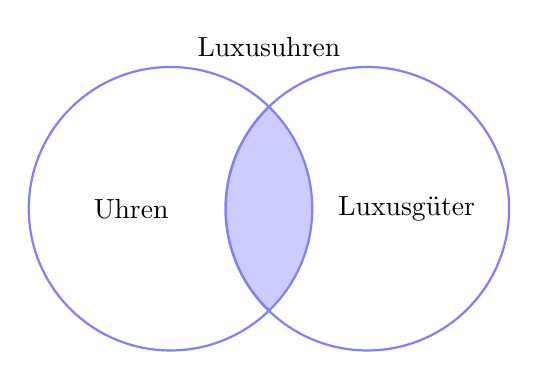
\begin{tikzpicture}
\begin{scope}
\clip \firstcircle;
\fill[filled] \secondcircle;
\end{scope}
\draw[outline] \firstcircle;
\node at (-0.5,0) {Uhren};
%
\draw[outline] \secondcircle;
\node at (3,0.0) {Luxusgüter};
%
\node[anchor=south] at (current bounding box.north) {Luxusuhren};
\end{tikzpicture}

\caption*{Veranschaulichung der Mengenbildung durch Schnitt von zwei Mengen.}
\end{framed}
\end{center}
\end{bsp}
\end{figure*}

\begin{bsp}\label{bsp:vereinSchnitt}~
\begin{enumerate}
\item $\N=\{n\in \N\mid n\text{ ist gerade}\}\cup \{n\in \N\mid n\text{ ist ungerade}\}$
\item $\varnothing=\{n\in \N\mid n\text{ ist gerade}\}\cap \{n\in \N\mid n\text{ ist ungerade}\}$
\item Sind $X_a$ und $X_b$ beliebige Mengen, dann gilt:
\[
X_a\cup X_b=\bigcup_{i\in\{a,b\}}X_i.
\]
\item Ist für jede natürliche Zahl $n$ die Menge $X_n$ als $\{0,\dots, n\}$ gegeben, dann gilt
\[
\bigcup_{n\in \N}X_n\,=\,\N
\]
und
\[
\bigcap_{n\in \N}X_n\,=\,\{0\}.
\]
\end{enumerate}
\end{bsp}


\begin{ueb}
    Beschreiben Sie folgende Mengen:
    \begin{enumerate}
        \item $\{0,2,4,\dots \}\cap \{p\in\N\mid p\text{ ist eine Primzahl} \}$
        \item $\N\cap\{\N\}$
        \item $\N\cup\{\N\}$
        \item $\{3x\mid x\in\N \} \cap \{5x\mid x\in\N \}$
    \end{enumerate}
    \begin{lsg}
        \ifthenelse{\boolean{ml}}
        {~
            \begin{enumerate}
                \item $\{2\}$
                \item $\varnothing$
                \item $\{\N,0,1,2,\dots \}$
                \item $\{15x\mid x\in\N \}$
            \end{enumerate}
        }{~
            \answerspace{3cm}}
    \end{lsg}
\end{ueb}

\begin{df}
 Zwei Mengen $X$ und $Y$ heissen \textit{disjunkt}, falls sie keine gemeinsamen Elemente haben, d.h. falls $X\cap Y=\varnothing$ gilt. Wir sagen eine Menge $\{X_i\mid i\in I \}$ von Mengen bestehe aus \textit{paarweise disjunkten} Mengen, wenn folgendes gilt:
 \[
 \forall i,j\in I\,(i\neq j\Rightarrow X_i\cap X_j=\varnothing).
 \]
\end{df}

\begin{figure*}[h]
   \begin{rk}\label{rk:disjunkt-paarweisedisjunkt}
       Für Mengen $\{X_i\mid i \in I \}$, hat die Annahme
       \[
           \bigcap_{i\in I}X_i=\varnothing
       \]
       nicht notwendigerweise zur Folge, dass die $X_i$'s paarweise disjunkt sind.
        \begin{center}
            \begin{framed}
                \def\firstcircle{(-4.5,2) circle (0.5cm)}
                \def\secondcircle{(-5.4,2) circle (0.5cm)}
                \def\thirdcircle{(-7,2) circle (0.5cm)}
                %
                \def\firstcircleA{(0,2) circle (0.5cm)}
                \def\secondcircleA{(1.1,2) circle (0.5cm)}
                \def\thirdcircleA{(2.2,2) circle (0.5cm)}
                %
                \colorlet{circle edge}{blue!50}
                \colorlet{circle area}{red!50}

                \tikzset{filled/.style={fill=circle area, draw=circle edge, thick},
                    outline/.style={draw=circle edge, thick}}

                \setlength{\parskip}{5mm}
                % Set A and B
                \begin{tikzpicture}
                \begin{scope}
                \clip \firstcircle;
                \fill[filled] \secondcircle;
                \end{scope}
                \draw[outline] \firstcircle node {$C$};
                \draw[outline] \secondcircle node {$B$};
                \draw[outline] \thirdcircle node {$A$};
                \node[anchor=south] at (1.2,0.8) {Paarweise disjunkt};
                %
                \draw[outline] \firstcircleA node {$A$};
                \draw[outline] \secondcircleA node {$B$};
                \draw[outline] \thirdcircleA node {$C$};
                %
                \node[anchor=south] at (-5.1,0.8) {Disjunkt ($A \cap B\cap C=\varnothing$),};
                \node[anchor=south] at (-5.3,0.3) {\textit{nicht} paarweise disjunkt};
                \end{tikzpicture}
            \end{framed}
        \end{center}
    \end{rk}
\end{figure*}


\begin{df}
 Sind $X$ und $Y$ beliebige Mengen, so definieren wir als
 \[
 X\setminus Y:=\{x\in X\mid x\notin Y\}
 \]
die Menge aller Elemente von $X$, die nicht zu $Y$ gehören. Die Menge $X\setminus Y$ nennt man ``$X$ ohne $Y$''. Ist eine ``Grundmenge'' $A$ (implizit oder explizit) vorgegeben, so bezeichnet man die Menge $A\setminus Y$ auch als ``Komplement'' oder ``Komplementärmenge'' von $X$ (relativ zu $A$).
\end{df}

\begin{bsp}
Die Menge der ungeraden Zahlen können wir als
\[
\N\setminus\{2x\mid x\in\N\}
\]
schreiben.
\end{bsp}

\begin{ueb}
Beschreiben Sie folgende Mengen.
\begin{enumerate}
\item $\N\setminus\{x\in\N\mid x \text{ ist gerade} \}$
\item $\{x\in\N\mid x\text{ ist gerade} \}\setminus \{3x\mid x\in \N \}$
\item $\N\setminus (\N\setminus \Z)$
\end{enumerate}
\end{ueb}
\begin{lsg}
\ifthenelse{\boolean{ml}}
{~
\begin{enumerate}
\item $\{x\in \N\mid x\text{ ist ungerade} \}$
\item Die Menge aller geraden und nicht durch $3$ teilbaren natürlichen Zahlen.
\item $\N$
\end{enumerate}
}
{~
\answerspace{4cm}}
\end{lsg}

\begin{satz}[Rechenregeln]
 Es gelten für beliebige Mengen $A,B$ und $C$ folgende Identitäten:
\begin{enumerate}
 \item Kommutativität der Vereinigung und des Schnittes:
\[
 A\cup B=B\cup A\text{ und }A\cap B=B\cap A.
\]
\item Assoziativgesetze von Schnitt und Vereinigung:
\[
 A\cap(B\cap C)=(A\cap B)\cap C\text{ und }A\cup(B\cup C)=(A\cup B)\cup C
\]

\item Distributivgesetze von $\cap$ mit $\cup$:
\[
 A\cap(B\cup C)=(A\cap B)\cup (A\cap C)\text{ und }A\cup(B\cap C)=(A\cup B)\cap (A\cup C)
\]
\item Idempotenzgesetz:
\[
 A\cap A=A\text{ und }A\cup A=A
\]
\item Regeln von DeMorgan:
\[
 (C\backslash A)\cap (C\backslash B)=C\backslash (A\cup B)\text{ und }(C\backslash A)\cup (C\backslash B)=C\backslash (A\cap B)
\]
\item Charakterisierung der Teilmengenbeziehung:
\[
A\subseteq B\Leftrightarrow A\cap B= A\Leftrightarrow A\cup B=B
\]
\end{enumerate}
\end{satz}
\begin{proof}[Beweis]
 Übung
\end{proof}


\begin{ueb}
Zeigen Sie für beliebige Mengen $A$ und $B$:
\begin{enumerate}
\item $A\setminus(A\setminus B)=A\cap B$
\item $(A\setminus B)\setminus B=A\setminus B$
\end{enumerate}
\end{ueb}
\begin{lsg}
\ifthenelse{\boolean{ml}}
{~
	\begin{enumerate}
	\item Es sei $x$ beliebig, es gilt:
	\begin{align*}
	x\in A\setminus (A\setminus B)&\Leftrightarrow x\in A\land (x\notin A\setminus B)\\
	&\Leftrightarrow x\in A\land \neg(x\in A\land x\notin B)\\
	&\Leftrightarrow x\in A\land (x\notin A\lor x\in B)\\
	&\Leftrightarrow (x\in A\land x\notin A)\lor (x\in A\land x\in B)\\
	&\Leftrightarrow x\in A\land x\in B\\
	&\Leftrightarrow x\in A\cap B
	\end{align*}
	\item Es sei $x$ beliebig, es gilt:
	\begin{align*}
	x\in (A\setminus B)\setminus B&\Leftrightarrow x\notin B\land (x\in A\setminus B)\\
	&\Leftrightarrow x\notin B\land (x\in A\land x\notin B)\\
	&\Leftrightarrow x\in A\land x\notin B\\
	&\Leftrightarrow x\in A\setminus B
	\end{align*}
	\end{enumerate}
}
{~
	\answerspace{8cm}
}
\end{lsg}

\begin{df}
Ist $A$ eine beliebige Menge, dann bezeichnen wir mit
\[
 \mathcal{P}(A):=\{x\mid x\subseteq A\}
\]
die \textit{Potenzmenge} von $A$, die genau die Teilmengen von $A$ als Elemente enthält.
\end{df}



\begin{bsp}
\begin{enumerate}
\item $\mathcal{P}(\varnothing)=\{\varnothing\}\neq \varnothing$
\item $\mathcal{P}(\{0,1\})=\big\{ \varnothing,\{0\},\{1\},\{0,1\} \big\}$
\end{enumerate}
\end{bsp}

\begin{ueb}~
Beschreiben Sie in aufzählender Form:
\begin{enumerate}
\item $\mathcal{P}(\{3,4\})$
\item $\mathcal{P}(\{a,\{c\}\})$
\item $\mathcal{P}(\{\{\{x\}\}\})$
\end{enumerate}
\end{ueb}
\begin{lsg}
\ifthenelse{\boolean{ml}}
{~
	\begin{enumerate}
	\item $ \{\varnothing, \{3\}, \{4\}, \{3, 4\}\} $
	\item $ \{\varnothing, \{a\}, \{\{c\}\}, \{a, \{c\}\}\} $
	\item $ \{\varnothing, \{\{\{x\}\}\}\} $
	\end{enumerate}
}
{~
\answerspace{4cm}
}
\end{lsg}

\begin{ueb}
Geben Sie Mengen $A$ und $B$ an, mit
\[
\mathcal{P}(A)\cup\mathcal{P}(B)\neq\mathcal{P}(A\cup B).
\]
\end{ueb}
\begin{lsg}
\ifthenelse{\boolean{ml}}{~
	z.B. $A=\{1,2\}$ und $B=\{2,3\}$
	}{~
	\answerspace{2.5cm}
	}
\end{lsg}

\begin{df}[Partitionen]\label{df:partition}
Eine \textit{Partition} $P=\{P_i\mid i\in I \}$ einer Menge $A$, ist eine Menge von Teilmengen von $A$, die folgende beiden Voraussetzungen erfüllt:
\begin{itemize}
\item Die Elemente von $P$ sind nichtleer und paarweise disjunkt.
\item $\bigcup_{i\in I}P_i=A$
\end{itemize}
Die Elemente einer Partition werden \textit{Blöcke} der Partition genannt.
\end{df}


\begin{bsp}~
\begin{itemize}
    \item Die Menge aller geraden natürlichen Zahlen und die Menge aller ungeraden natürlichen Zahlen bilden zusammen eine Partition der natürlichen Zahlen. Genauer, falls $G$ die Menge der geraden natürlichen Zahlen und $U$ die Menge der ungeraden natürlichen Zahlen ist, dann ist die Menge $\{G,U\}$ eine Partition von $\N$ mit zwei Blöcken.
    \item Für
    \begin{align*}
    A_i=\{i,-i\}
    \end{align*}
    ist die Menge $P=\{A_i\mid i\in\N\}$ eine Partition der Menge $\Z$ (in unendlich viele Blöcke).
\end{itemize}
\end{bsp}

\begin{ueb}~
\begin{enumerate}
\item Geben Sie eine Partition von $\N$ in unendlich viele Blöcke an.
\item Geben Sie eine Partition von $\N$ an, deren Blöcke alle unendlich gross sind.
\item Geben Sie eine Partition der rationalen Zahlen in unendlich viele, unendlich grosse
Blöcke an.
\end{enumerate}
\end{ueb}
\begin{lsg}
\ifthenelse{\boolean{ml}}{~
\begin{enumerate}
\item Z.B. $\{\{0\},\{1\},\dots \}$ also $\{P_i\mid i\in\N\}$ mit $P_i=\{i\}$.
\item Z.B. $\{P_1,P_2\}$ mit $P_1=\{x\in \N\mid x\text{ ist gerade} \}$ und $P_2=\{x\in \N\mid x\text{ ist ungerade} \}$.
\item Z.B. $ \{P_i\mid i\in \Z\}$ wobei $P_i=\{ x\in\Q\mid i<x\leq i+1 \}$.
\end{enumerate}}{~
\answerspace{6cm}}
\end{lsg}


\section{Relationen, Funktionen und Graphen}

Relationen beschreiben unterschiedlichste Beziehungen zwischen (mathematischen) Objekten. Vier völlig unterschiedliche Relationen könnten etwa wie folgt gegeben sein.
\begin{bsp}\label{ex:Beispiel1relationen}
Die Relationen $R_1,R_2,R_3$ und $T$ sind durch folgende Zuordnungen gegeben:
\begin{itemize}
\item Zwei Geraden stehen in Relation $R_1$ zueinander, wenn sie parallel sind. Dies ist eine (binäre) Relation auf der Menge aller Geraden.
\item Zwei Punkte auf der Erdoberfläche stehen zueinander in Relation $R_2$, wenn der erste Punkt zu Fuss (und ohne weitere Hilfsmittel) vom zweiten Punkt aus erreichbar ist.
\item Eine Person $P$ steht in Relation $R_3$ zu Person $Q$, wenn $P$ in $Q$ verliebt ist.
\item Eine natürliche Zahl $x$ steht in Relation $T$ zu einer natürlichen Zahl $y$, falls $x$ ein Teiler von $y$ ist.
\end{itemize}
\end{bsp}

Zum präziseren Formulieren von Relationen verwenden wir \textit{Tupel}, diese erlauben es uns beliebig Elemente zu kombinieren und in Beziehung zueinander zu setzten. \textit{Tupel} haben im Gegensatz zu Mengen mehr innere Struktur - die Reihenfolge und Wiederholung von Elementen sind wesentlich, sie sind gewissermassen die mathematische Entsprechung zu Listen und Arrays in der Informatik.

\begin{df}[Tupel]
Es sei $n>0$ eine natürliche Zahl. Ein $n$\textit{-Tupel} ist ein Term von der Form
\[
(x_1,\dots,x_n).
\]
Für beliebige Tupel gilt:
\[
(x_1,\dots,x_n)=(y_1,\dots y_k):\Leftrightarrow n=k\land x_1=y_1\land\dots\land y_n=x_n.
\]
$2$-Tupel nennen wir \textit{Paare} und $3$-Tupel \textit{Tripel}.
\end{df}

Die Gesamtheit aller Tupel mit Elementen aus einer oder mehreren gegebenen Mengen nennt man kartesisches Produkt.

\begin{df}\label{df:kartesischesProdukt}
Es seien $A_1,\dots, A_n$ Mengen und $n\in\N$ mit $n>0$.
Das \textit{kartesische Produkt} von $A_1,\dots, A_n$, ist die Menge aller $n$-Tupel mit Einträgen aus den Mengen $A_1,\dots ,A_n$:
\begin{align*}
\prod_{i=1}^{n}A_i=\big\{(a_1,\dots,a_n)\mid a_1\in A_1\land\dots\land a_n\in A_n \big\}.
\end{align*}
\end{df}

\begin{rk}
    Oft schreiben wir auch $A_1\times A_2\times \dots\times A_n$ für das kartesische Produkt $\prod_{i=1}^nA_i$. Insbesondere schreiben wir $X\times Y$ für das kartesische Produkt von zwei Mengen $X$ und $Y$, konkret heisst das:
    \[
    X\times Y:=\{(x,y)\mid x\in X\land y\in Y \}.
    \]
    Für das $n$-fache kartesisches Produkt $A\times A\times\dots\times A$ einer Menge $A$ mit sich selbst schreiben wir auch $A^n$.
    \end{rk}

    \begin{figure*}[h]
    \begin{bsp}
    Das kartesische Produkt der Menge $\N$ mit sich selbst enthält alle möglichen Paare von natürlichen Zahlen.
    \begin{center}
    \begin{framed}
    %
    \begin{tikzpicture}[dot/.style={circle,fill=black,minimum size=4pt,inner sep=0pt, outer sep=-1pt}]

    % horizontal axis
    \draw[->] (0,0) -- (5,0) node[anchor=north] {$\N$};
    % labels
    \draw	(3.5,0) node[anchor=north] {$14$};
    \draw	(-0.5,1.3) node[anchor=north] {$5$};
    \draw	(3.5,1) node[dot]{};
    \draw	(3.7,1.7) node[anchor=north]{$(14,5)$};

    % vertical axis
    \draw[->] (0,0) -- (0,3) node[anchor=east] {$\N$};
    % nominal speed
    \draw[dotted] (3.5,0) -- (3.5,1);
    \draw[dotted] (0,1) -- (3.5,1);
    \end{tikzpicture}
    %
    \caption*{Das Paar $(14,5)$ ist ein Element von $\N\times\N$.}
    \end{framed}
    \end{center}
    \end{bsp}
    \end{figure*}

    \begin{bsp}
        Die Menge der rationalen Zahlen
        \[
        \Q:=\left\{\frac{x}{y}\mid x\in \Z\land y\in\N\setminus\{0\}\right\}
        \]
        kann man als das kartesische Produkt
        \[
        \Z\times(\N\setminus\{0\})
        \]
        auffassen.
    \end{bsp}

Nun können wir Relationen mit Mengen von Tupeln, also Teilmengen von kartesischen Produkten, identifizieren. Wir erhalten dadurch einen sehr einfachen und allgemeinen Relationsbegriff, der beliebige (auch beliebig exotische) Beziehungen als Relationen zulässt.

\begin{df}
Eine $n$-stellige \textit{Relation} $R$ auf den Mengen $A_1,\dots A_n$ ist eine Menge von $n$-Tupeln aus $A_1\times\dots \times A_n$. Mit anderen Worten, die Relationen auf $A_1,\dots,A_n$ sind genau die Teilmengen
\begin{align*}
R\subseteq A_1\times\dots \times A_n.
\end{align*}
Ist $R$ eine $n$-stellige Relation und gilt $(x_1,\dots,x_n)\in R$, dann sagen wir, dass die Elemente $x_1,\dots,x_n$ zueinander in Relation $R$ stehen.
\end{df}

\begin{rk}
    Eine $2$-stellige Relation $R\subseteq X\times Y$ heisst auch eine \textit{binäre Relation} auf den Mengen $X$ und $Y$. Ist $R$ eine binäre Relation, so schreiben wir auch $xRy$ für $(x,y)\in R$.
\end{rk}

Wir werden uns im Folgenden auf binäre Relationen beschränken.

\begin{bsp}\label{Bsp:Geraden}
    Wir betrachten die Relation $R_1$ von Beispiel~\ref{ex:Beispiel1relationen} auf $\{g,h,p,q,r\}$. Die Geraden $g,h,p,q,r$ sind wie im folgenden Bild gegeben:
    \begin{center}
    %\begin{framed}
    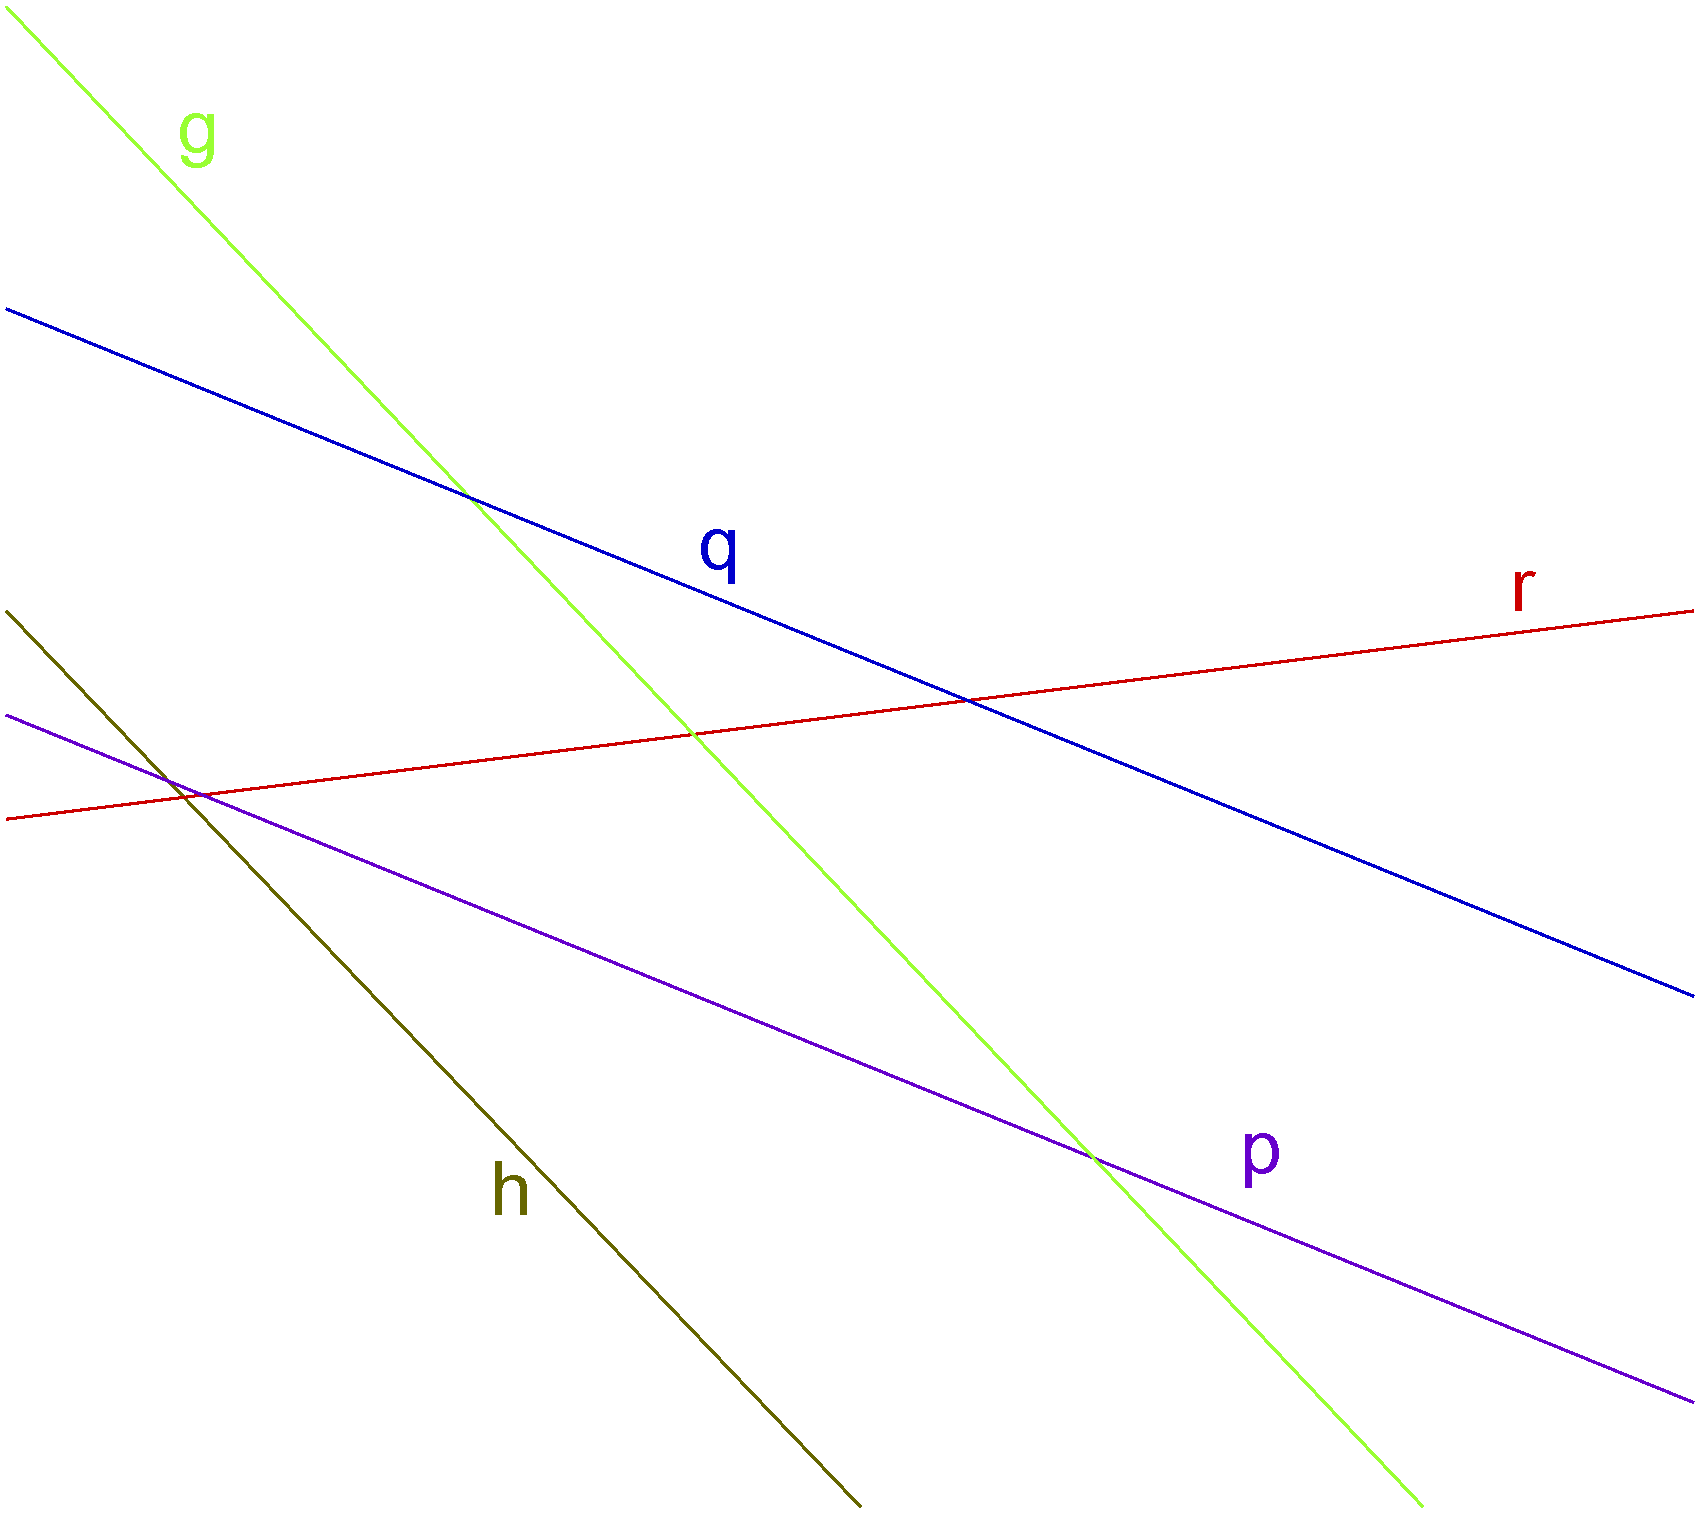
\includegraphics[width=0.5\linewidth]{images/figures/geraden}
    %\end{framed}
    \end{center}
    Offenbar gelten folgende Beziehungen:
    \begin{itemize}
    \item Die Gerade $g$ steht in Relation $R_1$ zu folgenden Geraden: $g$, $h$.
    \item Die Gerade $h$ steht in Relation $R_1$ zu folgenden Geraden: $g$, $h$.
    \item Die Gerade $p$ steht in Relation $R_1$ zu folgenden Geraden: $p$, $q$.
    \item Die Gerade $q$ steht in Relation $R_1$ zu folgenden Geraden: $p$, $q$.
    \item Die Gerade $r$ steht mit keiner anderen Geraden in Relation $R_1$.
    \end{itemize}
    Als Menge geschrieben, nimmt die Relation $R_1$ also folgende Gestalt an:
    \[
    R_1=\big\{(g,g),(g,h),(h,h),(h,g),(p,p),(p,q),(q,q),(q,p),(r,r)\big\}.
    \]
    Bildlich lässt sich die Relation als Tabelle darstellen:
    \begin{center}
    \begin{tabular}{ c | c c c c c }
    $r$&\xmark&\xmark&\xmark&\xmark&\cmark\\
    $q$&\xmark&\xmark&\cmark&\cmark&\xmark\\
    $p$&\xmark&\xmark&\cmark&\cmark&\xmark\\
    $h$&\cmark&\cmark&\xmark&\xmark&\xmark\\
    $g$&\cmark&\cmark&\xmark&\xmark&\xmark\\
    \hline
    &$g$&$h$&$p$&$q$&$r$
    \end{tabular}
    \end{center}
    Aus der Tabelle erhält man, ähnlich (gleich) wie im Fall von Funktionen und
    Funktionsgraphen, den Relationsgraph von $R_1$:
    \begin{center}
    \begin{tabular}{ c | c c c c c }
    $r$&&&&&\cellcolor{black}\\
    $q$&&&\cellcolor{black}&\cellcolor{black}&\\
    $p$&&&\cellcolor{black}&\cellcolor{black}&\\
    $h$&\cellcolor{black}&\cellcolor{black}&&&\\
    $g$&\cellcolor{black}&\cellcolor{black}&&&\\
    \hline
    &$g$&$h$&$p$&$q$&$r$
    \end{tabular}
    \end{center}
\end{bsp}

\begin{bsp}
    Der Relationsgraph der Teilbarkeitsrelation (die Relation
    $T$ von Beispiel~\ref{ex:Beispiel1relationen}) auf der Menge $\{n\in\N\mid 1<n<100 \}$.
    \begin{center}
    %\begin{framed}
    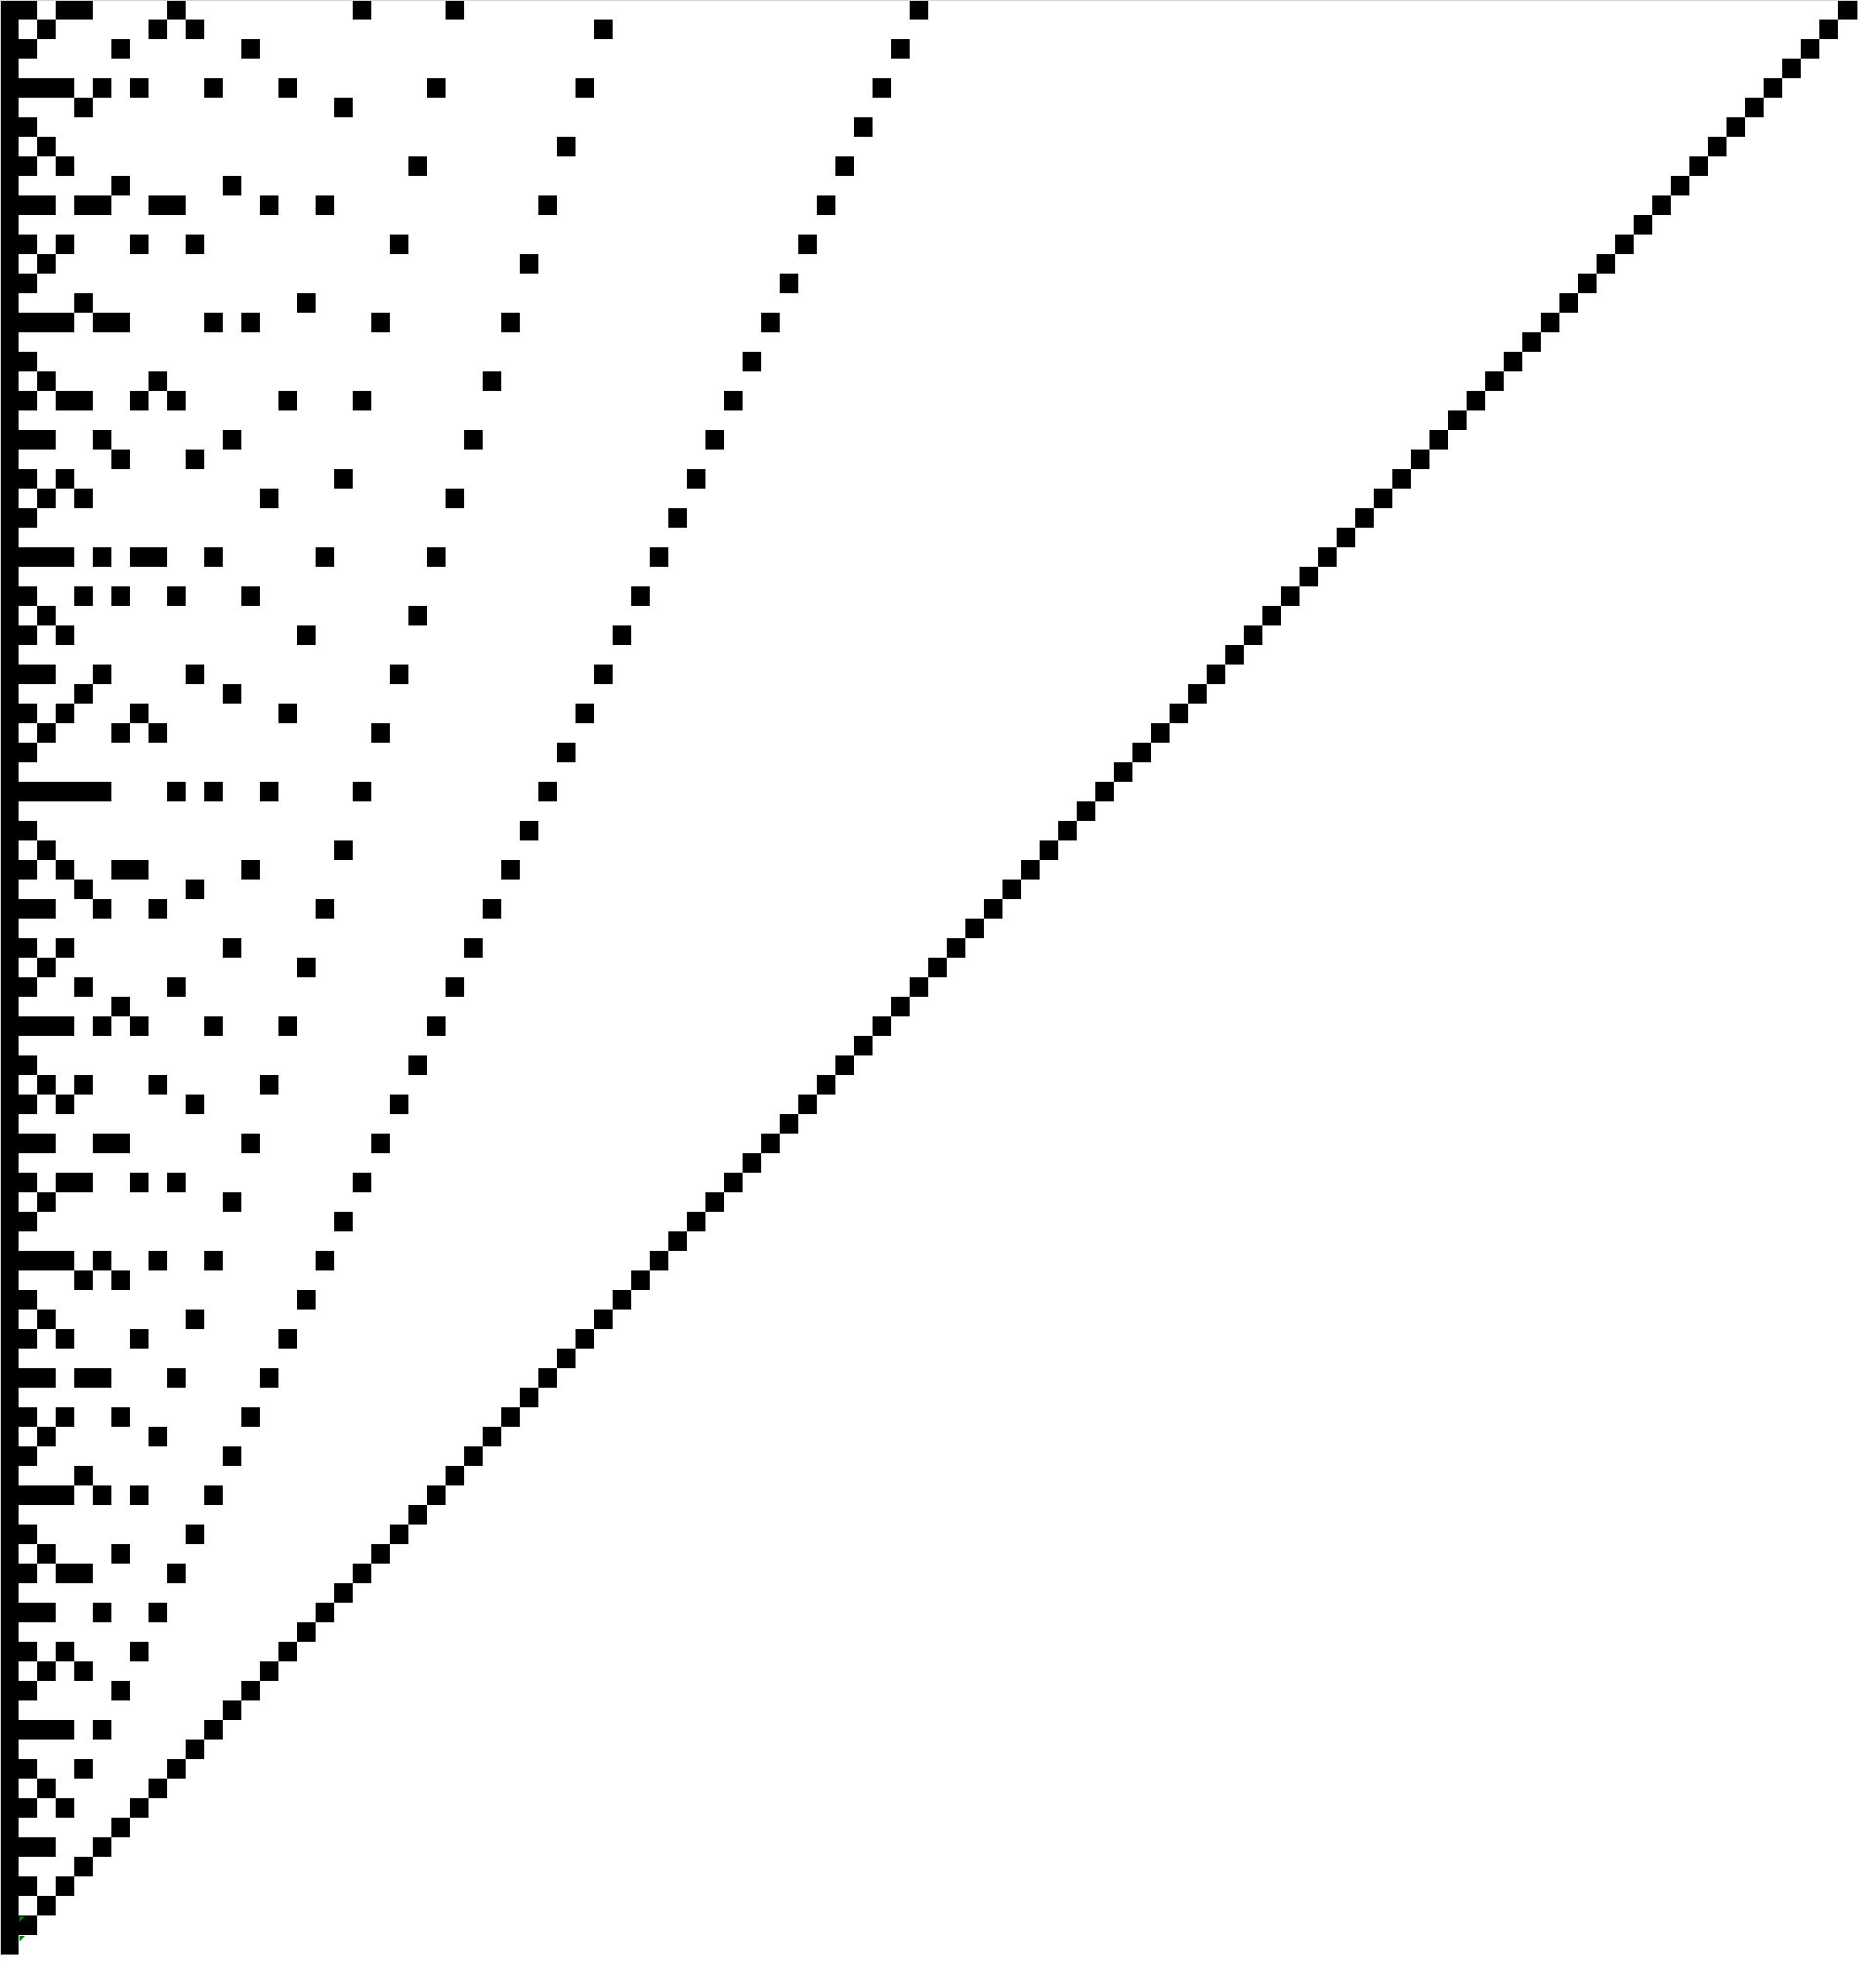
\includegraphics[width=0.3\linewidth]{images/figures/teiler}
    %\end{framed}
    \end{center}
    Der Relationsgraph von
    \[
    R=\{(x,y)\mid x,y\in\N\land x,y<100\land x+y\text{ ist ein Vielfaches von }7 \}
    \]
    \begin{center}
    %\begin{framed}
    
\includegraphics[width=0.3\linewidth]{images/figures/sum_modulo}
    %\end{framed}
    \end{center}
\end{bsp}


Ein alternativer Zugang zum Veranschaulichen von binären Relationen bietet die ``Graphentheorie''. Ein Graph\footnote{Nicht zu verwechseln mit einem Funktionsgraphen oder einem
Relationsgraphen} ist in diesem Kontext eine abstrakte Struktur bestehend aus Knoten und Verbindungen zwischen diesen Knoten (Kanten).

\begin{df}
    Ein \textit{(gerichteter) Graph} ist ein Paar $G=(V,E)$ bestehend aus einer Menge $V$ (Knotenmenge)
    und einer binären Relation $E\subseteq V\times V$ (Kantenmenge).
\end{df}

Endliche Graphen können grafisch dargestellt werden, dazu werden die Knoten durch Punkte oder Kreise und die Kanten durch Linien oder Pfeile zeichnerisch repräsentiert. Dies erlaubt es beliebige binäre Relationen zeichnerisch darzustellen.

\begin{bsp}
    Die Teilbarkeitsrelation auf der Menge $\{1,2,3,4\}$ lässt sich als Graph
    $G=(V,E)$ mit
    \begin{align*}
    V &= \{1,2,3,4\}\\
    E &= \{(1,1),(1,2),(1,3),(1,4),(2,2),(2,4),(3,3),(4,4)\}
    \end{align*}
    auffassen. Wir veranschaulichen den Graphen, indem wir die Knoten als Punkte oder Kreise
    und die Kanten als Pfeile zwischen den Knoten darstellen:

    \begin{center}
            \includegraphics[width=0.3\linewidth]{images/graphviz/g1.png}
    \end{center}


\end{bsp}

\begin{ueb}
    Stellen Sie die Relation $<$ auf der Menge $\{1,2,3,4\}$ als Graph dar.
\end{ueb}
\begin{lsg}~
    \ifthenelse{\boolean{ml}}{
        \begin{center}
            \includegraphics[width=0.3\linewidth]{images/graphviz/g2.png}
        \end{center}
    }
    {~\answerspace{5cm}}
\end{lsg}

\subsection{Funktionen}

Wichtige Vertreter von binären Relationen sind die \textit{Funktionen} wobei die grundlegende Idee einer Funktion im Verbinden von gewissen ``Inputelementen'' mit eindeutig bestimmten, dazu passenden, ``Outputelementen'' besteht. Konkret heisst dies:


\begin{itemize}
    \item Für jede Funktion gibt es eine klar definierte Menge von zulässigen ``Inputelementen'', dies nennt man die Definitionsmenge oder den Definitionsbereich der Funktion.
    \item Jedem ``Inputelement'' wird genau ein ``Outputelement'' zugeordnet. Jede Funktion ``produziert'' also für jeden zulässigen Input einen und nur einen (und stets den gleichen) Output.
\end{itemize}
Dies lässt sich wie folgt als mathematische Definition fassen.
\begin{df}
    Es seien $A$ und $B$ beliebige Mengen. Eine Relation $f\subseteq A\times B$ ist eine \textit{Funktion} von $A$ nach $B$, falls:
    \begin{align*}
    \forall x\in A\exists!y\in B((x,y)\in f)
    \end{align*}
    gilt. In diesem Fall schreiben wir
    \begin{align*}
    f:A\to B.
    \end{align*}
\end{df}

\begin{rk}
    Im Kontext einer Funktion $f:A\to B$ verwenden wir folgende Schreibweisen und Konventionen:
    \begin{itemize}
        \item Da zu jedem $x\in A$ ein eindeutig bestimmtes Element $y\in B$ mit $(x,y)\in f$ existiert, kann dieses $y$ mit $f(x)$ bezeichnet und \textit{Funktionswert von $f$ bei $x$} genannt werden.
        \item Die Menge aller Funktionswerte $Im(f) := \{f(x)\mid x\in A \}$ wird als \textit{Bild(menge)} von $f$ bezeichnet.
        \item Die Menge $A$ nennen wir den Definitionsbereich von $f$ und schreiben dafür auch $Dom(f)$.
        \item Der Definitionsbereich ist eindeutig durch die Funktion gegeben:
        \begin{align*}
            A=Dom(f)=\{x\mid \exists y ((x,y)\in f) \}=\{x\mid \exists y (f(x)=y )\}
        \end{align*}
        \item Die Menge $B$ ist durch die Voraussetzung $f:A\to B$ nicht eindeutig bestimmt, tatsächlich gilt $f:A\to B$ für jede Menge $B$ mit $Im(f)\subseteq B$.
    \end{itemize}
\end{rk}

\begin{rk}
    Oft werden Funktionen durch Spezifikation einer Definitions- und Zielmenge sowie einem Term für die ``Zuordnungsvorschrift'' oder ``Abbildungsvorschrift'' definiert. Die Funktion
    \begin{align*}
        f = \{(x,y)\in\N^2\mid y=x^2\}
    \end{align*}
    könnte etwa wie folgt angegeben werden:
    \begin{align*}
        f&:\N\to\N\\
        f&(x)=x^2
    \end{align*}
    Grundsätzlich gibt es keine Einschränkungen darüber wie eine Abbildungsvorschrift angegeben werden kann. Insbesondere lässt sich eine Funktion auf viele verschiedene Arten beschreiben\footnote{Man beachte die Unterscheidung zwischen einer Funktion (der Menge von geordneten Paaren) und ihrer Beschreibungen.}. Zur Veranschaulichung folgen zwei unterschiedliche Beschreibungen der Betragsfunktion:
    \begin{align*}
        |\cdot|&:\Z\to\Z\\
        |x| &= \sqrt{x^2}
    \end{align*}
    oder
    \begin{align*}
        |\cdot|&:\Z\to\Z\\
        |x| &= \begin{cases}
            -x&\text{wenn } x<0\\
            x&\text{sonst}
        \end{cases}
    \end{align*}
\end{rk}

\begin{ueb}
Geben Sie die Betragsfunktion wie oben definiert als Relation (Menge von geordneten Paaren) an.
\end{ueb}
\begin{lsg}
    \ifthenelse{\boolean{ml}}{
        Z.B.
        \begin{align*}
            \{(x,x)\mid x\in\N\}\cup\{(-x,x)\mid x\in\N\}
        \end{align*}
    }
    {~\answerspace{5cm}}
\end{lsg}

Funktionen lassen sich (bei geeigneten Definitions- und Bildmengen) kombinieren, man spricht dabei von der Komposition von Funktionen.

\begin{df}
    Sind $f:A\to B$ und $g:B\to C$ Funktionen, dann ist die Komposition $g$ nach $f$ durch
    \begin{align*}
        &g\circ f:A\to C\\
        (&g\circ f)(x)=g(f(x))
    \end{align*}
    gegeben.
\end{df}

Einige Funktionen ordnen nicht nur jedem Inputelement genau einen Output zu, sondern besitzen auch die ``umgekehrte Eigenschaft'', dass jeder Output nur mittels einem einzigen Inputelement erreicht werden kann. Derartige Funktionen nennt man \textit{injektiv}.

\begin{df}
    Eine Funktion $f$ ist genau dann \textit{injektiv}, wenn die Relation
    \begin{align*}
        f^{-1}=\{(y,x)\mid (x,y)\in f\}
    \end{align*}
    eine Funktion ist. Ist $f:A\to B$ eine injektive Funktion, dann nennt man $f^{-1}:Im(f)\to A$ die \textit{Umkehrfunktion} oder \textit{inverse Funktion} von $f$.
\end{df}


\begin{rk}
    Für $f:A \to B$ sind folgende Aussagen äquivalent.
    \begin{enumerate}
        \item Die Funktion $f$ ist injektiv
        \item Für alle $x,y\in A$ gilt: Aus $x\neq y$ folgt $f(x)\neq f(y)$
        \item Für alle $x,y\in A$ gilt: Aus $f(x)=f(y)$ folgt $x=y$
    \end{enumerate}
\end{rk}
\begin{proof}
    Die Aussagen in b) und c) sind offensichtlich äquivalent (Kontraposition). Für die Äquivalenz von $a)$ und $c)$ sei $f$ injektiv. Die Relation $f^{-1}=\{(y,x)\mid (x,y)\in f\}$ sei also eine Funktion. Daraus folgt, dass zu jedem $y$ höchstens ein $x$ mit $(y,x)\in f^{-1}$ existiert. Formal heisst das:
    \begin{align*}
        (y,x)\in f^{-1}\land (y,x')\in f^{-1}\Rightarrow x=x'
    \end{align*}
    Dies ist gleichbedeutend mit
    \begin{align*}
        (x,y)\in f\land (x',y)\in f\Rightarrow x=x'
    \end{align*}
    und somit
    \begin{align*}
        f(x)=y\land f(x')=y\Rightarrow x=x'
    \end{align*}
    was genau der Aussage in c) entspricht.
\end{proof}


Eine Funktion, die jedes Element einer gegebenen Zielmenge als Funktionswert realisiert, nennt man \textit{surjektiv auf der entsprechenden Zielmenge}.

\begin{df}
    Eine Funktion $f:A\to B$ heisst \textit{surjektiv} auf $B$, wenn $B=Im(f)$. Ist die Funktion $f$ zusätzlich injektiv, so sagen wir $f:A\to B$ sei \textit{bijektiv}.
\end{df}

\begin{wrn}
    So wie wir Funktionen eingeführt haben (als Mengen von geordneten Paaren) ist Surjektivität keine Eigenschaft, die eine Funktion für sich selbst genommen erfüllen kann. Nach dem hier gewählten Ansatz ist der Begriff der Surjektivität nur im Zusammenhang mit einer gegebenen Zielmenge sinnvoll. Andere Ansätze setzen voraus, dass jede Funktion bereits per Definition eine feste Zielmenge beinhaltet. In solchen Kontexten kann sinnvollerweise von surjektiven Funktionen gesprochen werden.
\end{wrn}

\begin{rk}
    Surjektivität und Injektivität lassen sich gut anhand von ``Gegenbeispielen'' veranschaulichen.
    Ist die Funktion $f: A\to B$ durch
    \begin{center}
        %\centering
    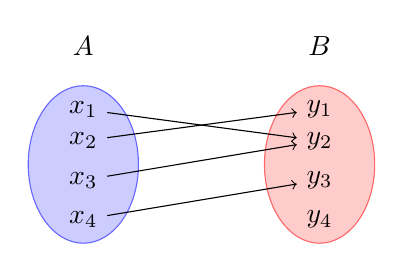
\begin{tikzpicture}
        % draw the sets
        \filldraw[fill=blue!20, draw=blue!60] (-1.5,0) circle [x radius=0.7cm, y radius=1cm];
        \filldraw[fill=red!20, draw=red!60] (1.5,0) circle [x radius=0.7cm, y radius=1cm];


        % the texts
        \node at (-1.5,1.5) {$A$};
        \node at (1.5,1.5) {$B$};

        % the points in the sets (here I just create nodes to use them later on to position
        % the circles and the arrows
        \node (x1) at (-1.5,0.7) {$x_1$};
        \node (x2) at (-1.5,0.3) {$x_2$};
        \node (x3) at (-1.5,-0.2) {$x_3$};
        \node (x4) at (-1.5,-0.7) {$x_4$};
        \node (y1) at (1.5,0.7) {$y_1$};
        \node (y2) at (1.5,0.3) {$y_2$};
        \node (y3) at (1.5,-0.2) {$y_3$};
        \node (y4) at (1.5,-0.7) {$y_4$};

        % draw the arrows
        \draw[->] (x1) -- (y2);
        \draw[->] (x2) -- (y1);
        \draw[->] (x3) -- (y2);
        \draw[->] (x4) -- (y3);

    \end{tikzpicture}
    \end{center}
    gegeben, dann gilt:
    \begin{itemize}
        \item Die Funktion ist wegen $f(x_1)=f(x_3)$ nicht injektiv.
        \item Die Funktion ist wegen $y_4\in B$ nicht surjektiv auf $B$.
        \item Die Funktion ist surjektiv auf $\{y_1,y_2,y_3\}$.
    \end{itemize}

\end{rk}

%Funktionen lassen sich bei Bedarf auf gewünschte Definitionsbereiche ``einschränken''.
%
%\begin{df}
%    Ist $f:A\to B$ eine Funktion und $X$ eine beliebige Menge, dann ist die \textit{Einschränkung} von $f$ auf $X$ wie %folgt gegeben:
%    \begin{align*}
%        &f\upharpoonright X:A\cap X\to B\\
%        &f\upharpoonright X(x)=f(x).
%    \end{align*}
%    Umgekehrt ist eine Funktion $g$ eine \textit{Erweiterung} von $f$, wenn $g\upharpoonright A= f$ gilt.
%\end{df}
%

\begin{lm}\label{lm: komposition inj surj}
    Für beliebige Funktionen $f:X\to Y$ und $g:Y\to Z$ gelten folgende Aussagen:
    \begin{enumerate}
        \item Falls $f:X\to Y$ und $g:Y\to Z$ injektiv sind, dann ist auch $g\circ f:X\to Z$ injektiv.
        \item Falls $f:X\to Y$ und $g:Y\to Z$ surjektiv sind, dann ist auch $g\circ f:X\to Z$ surjektiv.
    \end{enumerate}
\end{lm}
\begin{proof}
    \begin{enumerate}
        \item Wir nehmen an, dass $f:X\to Y$ und $g:Y\to Z$ injektiv sind und zeigen, dass $g\circ f:X\to Z$ injektiv ist. Es seien $a,b\in X$ verschiedene Elemente. Weil $f$ injektiv ist, folgt $f(a)\neq f(b)$ und folglich aus der Injektivität von $g$, wie gewünscht
        \begin{align*}
            g\circ f(a) = g(f(a))\neq g(f(b))=g\circ f(b).
        \end{align*}
        \item Für die zweite Behauptung müssen wir zeigen, dass zu jedem $z\in Z$ ein $x\in X$ existiert mit $g(f(x))= z$. Es sei also $z\in Z$ beliebig. Weil $g:Y\to Z$ surjektiv ist, gibt es ein $y\in Y$ mit $g(y)=z$. Weil $f:X\to Y$ ebenfalls surjektiv ist, gibt es weiter ein $x\in X$ mit $f(x) = y$. Insgesamt haben wir wie gewünscht
        \begin{align*}
            g(f(x))=g(y)=z.
        \end{align*}
    \end{enumerate}
\end{proof}

Eine wichtige Anwendung vom Funktionsbegriff innerhalb der Mengenlehre besteht darin mithilfe von Funktionen unendlich grosse Mengen (z.B. $\N$, $\Z$, etc.) miteinander bezüglich ihrer Grösse zu vergleichen.

\subsection{Grössenvergleiche von unendlichen Mengen}

Bevor wir uns mit unendlichen Mengen befassen, sollten wir uns darüber im Klaren sein, dass unser ``gesunder Menschenverstand'' ein gefährlicher Begleiter auf diesem Weg sein kann. Um zu sehen, wie heikel die Vermischung von alltäglichen Konzepten mit der Vorstellung des Unendlichen sind, betrachten wir ein Hotel mit unendlich vielen Zimmern -- das sogenannte Hilbert Hotel.
\begin{bsp}[Hilbert's Hotel]
Hilbert's Hotel hat unendlich viele Zimmer, für jede natürliche Zahl eines.
\begin{center}
\begin{framed}
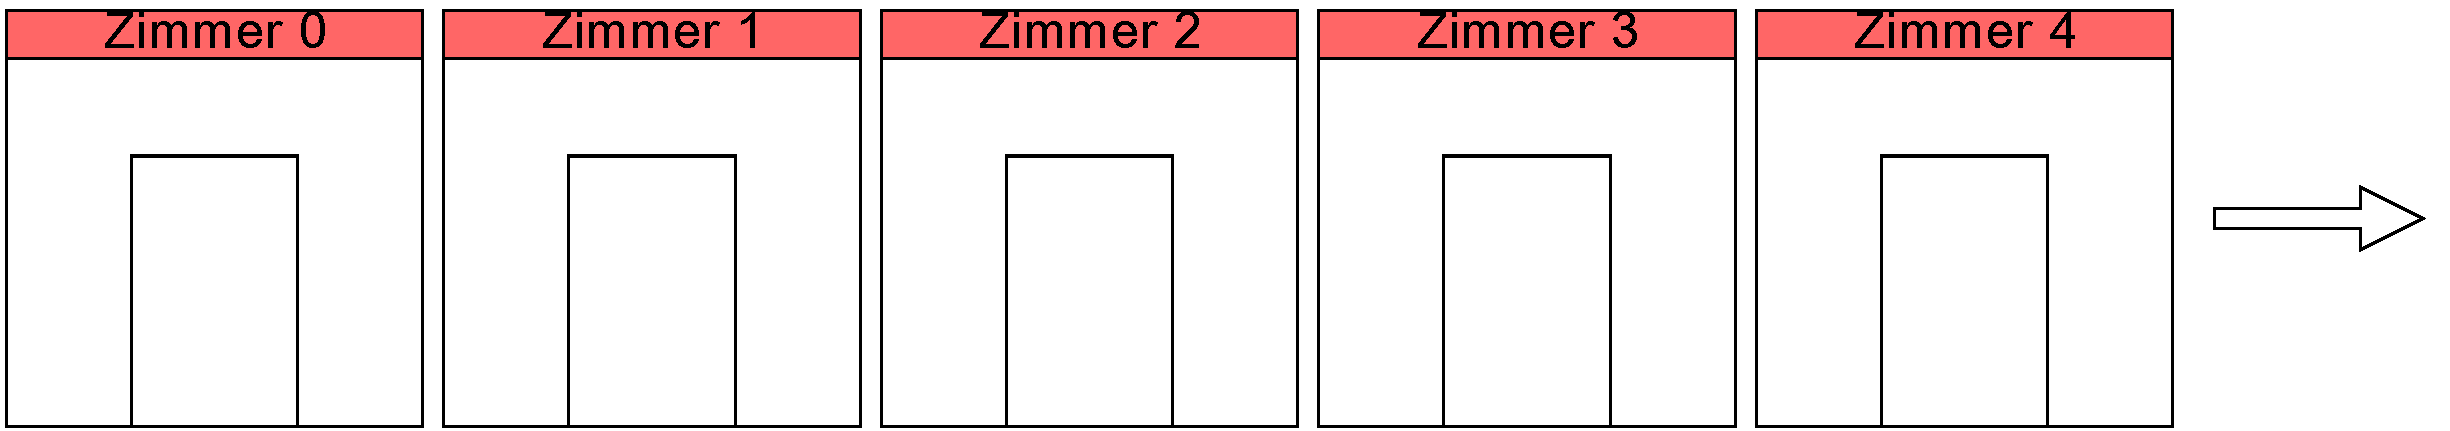
\includegraphics[width=0.9\linewidth]{images/figures/hilbertHotel}
%\caption*{Hilbert's Hotel}
\end{framed}
\end{center}
Im Rahmen eines Ferienjobs haben Sie eine Stelle als Concierge in Hilbert's Hotel angenommen\footnote{Sie verdienen schliesslich für jedes Zimmer einen Franken pro Arbeitstag.}. An Ihrem ersten Arbeitstag haben Sie die Nachtschicht. Herr Hilbert, der Hotelbesitzer, hat sich bereits zu seinem wohlverdienten Feierabend verabschiedet, als unvermittelt ein älterer Herr (ä.H.) die Lobby betritt.
\begin{itemize}
\item[ä.H.:] Ich bräuchte ein Zimmer in Ihrem Hotel.
\item[Sie:] Es tut mir leid, wir sind voll belegt. Ich könnte Ihnen aber das Hotel ``Cantors Paradise'' empfehlen. Es ist hier ganz in der Nähe, hier steht die Adresse.

\textit{Sie überreichen dem ä.H. eine Visitenkarte vom ``Cantors Paradise''.}
\item[ä.H.:] Mein lieber Concierge, laut Werbebroschüre hat Ihr Hotel unendlich viele Zimmer. Wie soll denn das bitte ausgebucht sein?
\item[Sie:] Na ja, wir haben im Moment unendlich viele Gäste -- in jedem Zimmer einen.
\item[ä.H.:] Das lass ich mal Ihr Problem sein! Mir genügt es, dass hier schwarz auf weiss steht, dass man angeblich keine Reservation zu tätigen braucht, um in diesem Hotel unterzukommen. Zudem werben Sie, mit Bezugnahme auf die Unendlichkeit Ihres Hotels, damit, dass jedem Gast und zu jeder Zeit ein Zimmer garantiert werden kann!

\textit{Der ä.H. kramt genervt seine Werbebroschüre hervor und zeigt sichtlich irritiert auf die entsprechende Seite.}
\item[Sie:] Hmm, ich werde sehen, ob sich da vielleicht doch was machen lässt. Bitte gedulden Sie sich einen Moment.

\textit{Der ä.H. lässt sich auf die grosse Couch fallen, die in der Eingangshalle steht. Sie, nicht ohne ein ziemlich ungutes Gefühl dabei zu haben, wählen Hilberts private Telefonnummer.}
\item[Hi.:] Hilbert am Apparat.
\item[Sie:] Entschuldigen Sie die späte Störung Herr Hilbert. Es ist mir unendlich unangenehm, aber ich habe hier im Hotel ein Problem.
\item[Hi.] Worum geht es denn?
\item[Sie:] Ich habe einen Gast, der trotz Vollbelegung auf ein Zimmer besteht. Und er kann sich erst noch auf unsere eigene Broschüre stützen, in der ja steht, dass wir nie ausgebucht seien, selbst dann nicht, wenn wir mal voll sein sollten!
\item[Hi.:] Ach ja, ich hatte vergessen Sie darauf aufmerksam zu machen. Alle unsere Gäste haben sich beim Bezug ihres Zimmers, {\tiny im Kleingedruckten}, damit einverstanden erklärt, dass wir sie im Notfall ein einziges Mal umplatzieren können. Nutzen Sie diese Klausel um unserem Gast ein Zimmer freizumachen. Noch etwas, machen Sie das Zimmer so frei, dass sie weitere Gäste, die vielleicht später noch kommen, ebenfalls noch unterbringen könnten und bedenken Sie stets, dass jeder Gast höchstens einmal umplatziert werden darf.

\textit{Sie beenden das Gespräch und wenden sich dem ungeduldig wartenden ä.H. zu.}
\item[Sie:] Sehr geehrter Herr, wir haben ein Zimmer für Sie gefunden, sie müssen sich bloss zwei Minuten gedulden, dann können Sie einziehen.
\item[ä.H.:] Sehen Sie, geht doch!
\end{itemize}
Wie bringen Sie den ä.H. unter? Bringen Sie weitere Gäste unter? Was machen Sie, wenn ein voller Limesbus (ein Bus mit unendlich vielen Sitzplätzen) ankommt? Wie lange dauert es bis der ganze Limesbus untergebracht wird?
\end{bsp}

\begin{df}\label{df:endlabzusw}~
\begin{itemize}
\item Eine Menge $X$ heisst \textit{endlich}, falls $X=\varnothing$ oder eine natürliche Zahl $n\geq 1$ und eine bijektive Funktion $f:X \to \{1,\dots,n\}$ existieren.
Ist $X\neq\varnothing$ eine endliche Menge, dann existiert eine Darstellung der Form $X=\{x_1,x_2,\dots,x_n\}$ wobei die Elemente $x_i$ paarweise verschieden sind (d.h. es gilt $i\neq j\Rightarrow x_i\neq x_j$). In diesem Fall hat die Menge $X$ genau $n$ viele Elemente und wir schreiben $|X|=n$. Weiter schreiben wir $|\varnothing| = 0$.
\item Nicht endliche Mengen nennen wir \textit{unendlich}.
\item Eine Menge $X$ heisst \textit{abzählbar}, wenn eine surjektive Funktion $F:\N\to X$ existiert oder wenn $X=\varnothing$ gilt.
\item Die Menge $X$ heisst \textit{abzählbar unendlich}, wenn $X$ abzählbar und unendlich ist.
\item Eine \textit{überabzählbare} Menge ist eine Menge, die nicht abzählbar ist.
\end{itemize}
\end{df}

\begin{rk}\label{rk:abzMengeAnschauung}
Ähnlich wie im Fall von endlichen Mengen ist jede nichtleere abzählbare Menge $X$ von der Form
\[
X=\{a_0,a_1,a_2,\dots \}=\{a_i\mid i\in\N\}.
\]
Den Zusammenhang zu Definition~\ref{df:endlabzusw} liefert hier die Funktion $F:\N\to X$, die durch $F(i)=a_i$ gegeben ist.
\end{rk}
\begin{rk}
Abzählbare Mengen kann man sich auch als die Mengen vorstellen, deren Elemente von den natürlichen Zahlen durchnummeriert  (Wiederholungen erlaubt) werden können. Die Elemente einer abzählbaren Menge lassen sich also in eine Liste schreiben, die für jede natürliche Zahl eine Zeile hat.
\begin{center}
\begin{tabular}{c|c}
$\N$ & $X$\\
\hline
$0$ & $x$\\
$1$ & $y$\\
$2$ & $z$\\
$\vdots$ & $\vdots$
\end{tabular}
\end{center}
\end{rk}

\begin{lm}[Schubfachprinzip]
    Wenn $n$ Objekte auf $m$ Behälter verteilt werden und $n>m$ gilt, dann gibt es mindestens einen Behälter, der mehr als ein Objekt enthält. Formal, sind $n>m$ natürliche Zahlen und gelte $|X|= n$ sowie $|Y|=m$, dann gibt es keine injektive Funktion
    \begin{align*}
    F: X\to Y.
    \end{align*}
\end{lm}

\begin{ueb}~

    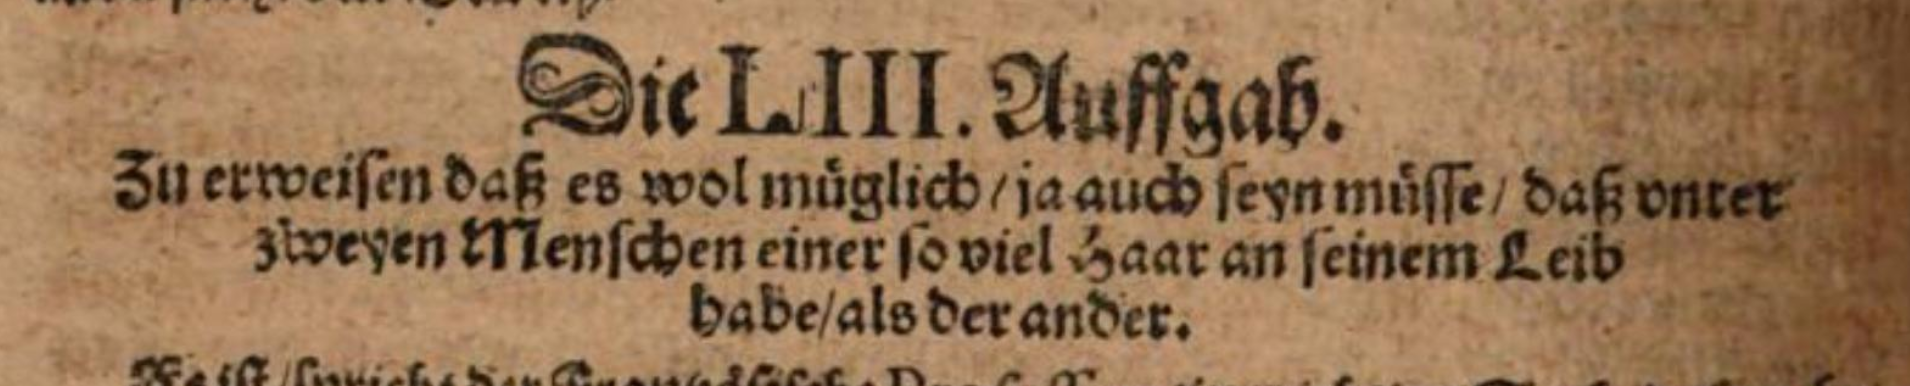
\includegraphics[width=0.9\linewidth]{images/figures/historicPigeon.png}
\end{ueb}
\begin{lsg}
    \ifthenelse{\boolean{ml}}{
        Wir teilen die Menge aller Menschen wie folgt in Gruppen $G_0,G_1,\dots$ ein
    \begin{align*}
    G_i=\text{ Alle Menschen, die genau $i$ viele Haare am Körper haben.}
    \end{align*}
    Weil jeder Mensch definitiv weniger als $10$ Mio. Haare besitzt (vgl. \url{https://bionumbers.hms.harvard.edu/bionumber.aspx?id=101509}) und weil definitiv mehr als $10$ Mio. Menschen existieren, können wir gemäss dem Schubfachprinzip darauf schliessen, dass es mindestens eine Gruppe mit mehreren Menschen darin gibt (also Menschen mit exakt der gleichen Anzahl an Haaren).
    \vspace{1cm}}{
        ~\answerspace{6cm}
    }
\end{lsg}

\begin{lm}\label{injEndl}
    Gibt es eine injektive Funktion $F:\N\to A$, dann ist die Menge $A$ unendlich.
\end{lm}
\begin{proof}
    Es sei eine Menge $A$ und eine injektive Funktion $F:\N\to A$ gegeben. Wäre die Menge $A$ endlich, dann gäbe es eine natürliche Zahl $n$ mit $|A|=n$. Die Funktion
    \begin{align*}
    G&:\{0,\dots,n\}\to A\\
    G&(x) = F(x)
    \end{align*}
    wäre injektiv und würde, wegen $|\{0,\dots,n\}|=n+1$, dem Schubfachprinzip widersprechen.
\end{proof}

\begin{satz}
    Folgende Aussagen sind für unendliche Mengen $A$ äquivalent:
    \begin{enumerate}
        \item Die Menge $A$ ist abzählbar.
        \item Es gibt eine surjektive Funktion $F_{\N,A}:\N\to A$.
        \item Es gibt eine injektive Funktion $F_{A,\N}:A\to\N$.
        \item Es gibt eine bijektive Funktion $B_{\N,A}:\N\to A$.
        \item Es gibt eine bijektive Funktion $B_{A,\N}:A\to\N$.
    \end{enumerate}
\end{satz}
\begin{proof}~
    \begin{itemize}
        \item Die Aussagen in $a)$ und $b)$ sind per Definition äquivalent.
        \item Die Aussagen in $d)$ und $e)$ sind offensichtlich äquivalent (Umkehrfunktion).
        %\item Für die Implikation $b)\Rightarrow c)$ definieren wir
        %\begin{align*}
        %    F_{A,\N}(a)=\min\{n\in\N \mid F_{\N,A}(n)=a\},
        %\end{align*}
        %dies ist gerechtfertigt\footnote{Wir gehen hier davon aus, dass jede nichtleere Menge von natürlichen Zahlen ein kleinstes Element besitzt, eine Tatsache die wir später beweisen werden.}, da aus der Surjektivität von $F_{\N,A}:\N\to A$ folgt, dass zu jedem $a\in A$ mindestens ein $n\in\N$ mit $F_{\N,A}(n)=a$ existiert. Es bleibt die Injektivität von $F_{A,\N}$ nachzuweisen, dazu nehmen wir $F_{A,\N}(a)=F_{A,\N}(a')$ an. Es folgt, dass es eine natürliche Zahl $n$ mit $F_{\N,A}(n)=a$ und $F_{\N,A}(n)=a'$ gibt. Somit muss wie gewünscht $a=a'$ gelten.
        \item Für die Implikation $c)\Rightarrow b)$, gehen wir von einer injektiven Funktion $F_{A,\N}:A\to\N$ aus.
        Weil diese Funktion injektiv ist, und weil $Dom(F_{A,\N})=A$ gilt, ist
        \begin{align*}
            F_{A,\N}^{-1}:Im(F_{A,\N}) \to A
        \end{align*}
        eine surjektive Funktion. Um eine surjektive Funktion von $\N$ nach $A$ zu erhalten, brauchen wir bloss noch die ``restlichen'' Elemente aus $\N$ zuzuordnen, dazu wählen wir ein beliebiges Element aus $a\in A$ und setzen:
        \begin{align*}
            F_{\N,A}(n)=
                \begin{cases}
                F_{A,\N}^{-1}(n)&\text{falls }n\in Im(F_{A,\N})\\
                a&\text{sonst}
                \end{cases}
        \end{align*}
        \item Für die Implikation $b)\Rightarrow d)$ müssen wir, ausgehend von einer unendlichen Menge $A$ und einer surjektiven Abbildung $F_{\N,A}: \N\to A$, eine bijektive Abbildung $B_{\N,A}: \N\to A$ konstruieren. Da uns für einen vollständigen Beweis die Werkzeuge noch fehlen (Rekursion), wollen wir hier bloss eine Beweisskizze präsentieren. Wir definieren die Funktion $B_{\N,A}$ rekursiv wie folgt:
        \begin{align*}
        B_{\N,A}(0) &= F_{\N,A}(0)\\
        B_{\N,A}(n+1) &= F_{\N,A}(\min\{k\in\N\mid F(k)\neq B_{\N,A}(0),\dots,B_{\N,A}(n) \})
        \end{align*}
        Die resultierende Funktion ist auf ganz $\N$ definiert, weil die Menge $A$ unendlich ist (würde die Rekursion abbrechen, dann wäre $A$ von der Form $\{F_{\N,A}(0),\dots,F_{\N,A}(m)\}$ für ein $m\in\N$). Die Funktion $B_{\N,A}$ ist surjektiv, weil $F_{\N,A}$ surjektiv ist. Die Injektivität folgt, weil per Konstruktion für alle $x,y$
        \begin{align*}
        x<y \Rightarrow B_{\N,A}(x) \neq B_{\N,A}(y)
        \end{align*}
        gilt.
    \end{itemize}
    Weil aus $d)$ und $e)$ alle anderen Aussagen direkt folgen, genügen die gezeigten Implikationen für den Beweis des Satzes.
\end{proof}

\begin{ueb}
    Die Funktion
    \begin{align*}
        &f :\N\to\N\\
        &f(x) =
            \begin{cases}
                \frac{x}{2}&\text{falls $x$ gerade}\\
                3x+1&\text{sonst}
            \end{cases}
    \end{align*}
    Ist surjektiv aber nicht injektiv. Wenn Sie die Funktion so wie im vorhergehenden Beweis im Schritt von $F_1$ zu $B_{\N,A}$ anpassen, welchen Funktionswert erhalten Sie dann für die Eingabe $8$?
\end{ueb}
\begin{lsg}~
    \ifthenelse{\boolean{ml}}{
        $f(9)=28$
    }{
        ~\answerspace{0cm}
    }
\end{lsg}

\begin{bsp}
Die Menge aller geraden natürlichen Zahlen ist abzählbar.
\begin{proof}
Ist $G$ die Menge der geraden Zahlen, dann folgt die Behauptung aus der Tatsache, dass die Funktion
\[
F:\N\to G \phantom{abstand}\text{ mit }\phantom{abstand}F(n)=2n
\]
jede gerade natürliche Zahl trifft (und somit surjektiv ist).
\end{proof}
Dass die Menge der geraden natürlichen Zahlen auch anschaulich abzählbar ist, kann man sich etwa mit folgender Auflistung vergegenwärtigen:
\begin{center}
\begin{tabular}{c|c}
$\N$ & $G$\\
\hline
$0$ & $0$\\
$1$ & $2$\\
$2$ & $4$\\
$\vdots$ & $\vdots$
\end{tabular}
\end{center}
\end{bsp}

\begin{bsp}
Die Menge $\Z$ der ganzen Zahlen ist abzählbar.
\begin{proof}
Wir müssen eine Funktion $F:\N\to\Z$ angeben, die jedes Element von $\Z$ trifft. Dies gelingt uns wie folgt:
\begin{align*}
F(n)=\begin{cases}
-\frac{n}{2} &\text{falls $n$ gerade}\\
\frac{n+1}{2}&\text{falls $n$ ungerade. }
\end{cases}
\end{align*}
\end{proof}
Anschaulich ergibt sich durch die Funktion $F$ folgende Auflistung der ganzen Zahlen:
\begin{center}
\begin{tabular}{c|c}
$\N$ & $\Z$\\
\hline
$0$ & $0$\\
$1$ & $1$\\
$2$ & $-1$\\
$3$ & $2$\\
$4$ & $-2$\\
$5$ & $3$\\
$\vdots$ & $\vdots$
\end{tabular}
\end{center}
\end{bsp}

\begin{bsp}
Die Menge aller \textit{endlichen} Sequenzen der Buchstaben $a,b$ ist abzählbar unendlich. Eine mögliche Auflistung der endlichen Sequenzen ist etwa durch
\begin{center}
\begin{tabular}{c|c}
$\N$ & $X$\\
\hline
$0$ & $a$\\
$1$ & $b$\\
$2$ & $aa$\\
$3$&$ab$\\
$4$&$ba$\\
$5$&$bb$\\
$6$&$aaa$\\
$7$ & $aab$\\
$8$ & $aba$\\
$9$ & $abb$\\
$\vdots$ & $\vdots$
\end{tabular}
\end{center}
gegeben.
\end{bsp}
\begin{bsp}
Die Menge aller Java, C, C\#, C++,Fortran\dots Programme ist abzählbar.
\end{bsp}
\begin{proof}
Wenn jedes Programm mit seinem Bytecode identifiziert wird, dann entspricht jedes Programm einer endlichen $0,1$-Folge. Diese können, gleich wie endliche $a,b$-Sequenzen, abgezählt werden.
\end{proof}
\begin{satz}
Jede endliche Menge ist abzählbar.
\end{satz}
\begin{proof}
Ist $X$ eine endliche Menge, dann können wir $X$ als $\{x_1,\dots,x_n\}$ mit einer natürlichen Zahl $n$ schreiben. Da die leere Menge per Definition abzählbar ist, können wir annehmen, dass $X$ mindestens ein Element $x_1$ besitzt. Wir definieren nun die Funktion $F:\N\to X$ mit
\begin{align*}
F(i)=\begin{cases}
x_i&\text{falls }0<i\leq n\\
x_1&\text{sonst.}
\end{cases}
\end{align*}
Da $F$ offensichtlich jedes Element von $X=\{x_1\dots x_n\}$ trifft, ist $F$ surjektiv. Somit ist $X$ abzählbar.
\end{proof}

\begin{satz}
Jede Teilmenge einer abzählbaren Menge ist abzählbar.
\end{satz}
\begin{proof}
Es sei $X\subseteq Y$ und $Y$ sei eine abzählbare Menge. Da $Y$ abzählbar ist,
gibt es eine surjektive Funktion $F:\N\to Y$. Wenn $X=\varnothing$ gilt, dann
ist $X$ per Definition abzählbar und wir sind fertig. Ist $X\neq\varnothing$,
dann gibt es ein Element $a\in X$. Wir können nun wie folgt eine Abbildung
$G:\N\to X$ angeben.
\begin{align*}
G(x)=\begin{cases}
F(x)&\text{falls }F(x)\in X\\
a&\text{sonst.}
\end{cases}
\end{align*}
Da $X\subseteq Y$ gilt und weil jedes Element von $Y$ von der Funktion $F$
getroffen wird, wird auch jedes Element von $X$ von $G$ getroffen. Somit
ist $G:\N\to X$ surjektiv und $X$ ist also abzählbar.
\end{proof}

\begin{satz}\label{satz:abzaehlbarTransitiv}
Ist $X$ eine abzählbare Menge und gibt es eine surjektive Funktion $F:X\to Y$, dann ist auch $Y$ abzählbar.
\end{satz}
\begin{proof}
Diese Behauptung folgt sofort aus Lemma \ref{lm: komposition inj surj} (die Komposition von surjektiven Funktionen ist wieder surjektiv).
%Sollte $X$ die leere Menge sein, dann ist auch $Y$ leer und somit abzählbar. Ist $X$ nichtleer, dann folgt aus der Abzählbarkeit von $X$, dass es eine surjektive Abbildung $G:\N\to X$ gibt. Wir können nun die Funktion $H:\N\to Y$ durch Komposition der Funktionen $F$ und $G$ bilden, d.h. wir definieren
%\begin{align*}
%H:\N\to Y\phantom{abstand}\text{ mit }\phantom{abstand} H(n)=F(G(n)).
%\end{align*}
%Wir müssen nun noch zeigen, dass wir mit der Funktion $H$ jedes Element von $Y$ treffen. Wir nehmen dazu ein beliebiges Element $y$ von $Y$ und zeigen, dass es eine natürliche Zahl $n$ gibt mit $H(n)=y$. Es sei also $y\in Y$ beliebig. Da die Funktion $F:X\to Y$ surjektiv ist, muss es ein $x\in X$ geben so, dass $F(x)=y$ gilt. Weil aber auch die Funktion $G:\N\to X$ surjektiv ist, muss es ebenfalls eine natürliche Zahl $n$ geben, mit $G(n)=x$. Zusammenfassend können wir also sagen, dass es eine natürliche Zahl und ein Element $x$ aus $X$ gibt, mit der Eigenschaft
%\[
%H(n)=F(G(n))=F(x)=y.
%\]
%Weil $y\in Y$ beliebig gewählt wurde, ist die Funktion $H$ surjektiv.
\end{proof}



\begin{satz}[Erstes Diagonalargument]\label{cantor1}
Die Menge $\N\times\N$, bestehend aus allen Paaren von natürlichen Zahlen, ist abzählbar.
\end{satz}
\begin{proof}[Beweisidee]
Anstelle eines formalen Beweises, skizzieren wir eine Abzählung aller Paare von natürlichen Zahlen wie folgt:
%\begin{figure}[h!]
\begin{center}
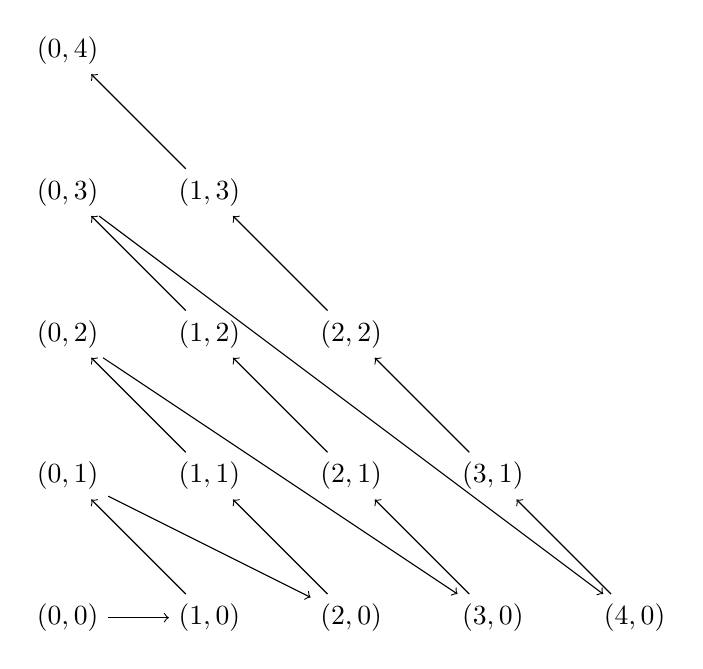
\begin{tikzpicture}[scale=1.8]
\node (0) at (0,0) {$(0,0)$};
\node (2) at (0,1) {$(0,1)$};
\node (5) at (0,2) {$(0,2)$};
\node (9) at (0,3) {$(0,3)$};
\node (14) at (0,4) {$(0,4)$};
\node (1) at (1,0) {$(1,0)$};
\node (4) at (1,1) {$(1,1)$};
\node (8) at (1,2) {$(1,2)$};
\node (13) at (1,3) {$(1,3)$};
\node (3) at (2,0) {$(2,0)$};
\node (7) at (2,1) {$(2,1)$};
\node (12) at (2,2) {$(2,2)$};
\node (6) at (3,0) {$(3,0)$};
\node (11) at (3,1) {$(3,1)$};
\node (10) at (4,0) {$(4,0)$};
\draw[->] (0) -- (1);
\draw[->] (1) -- (2);
\draw[->] (2) -- (3);
\draw[->] (3) -- (4);
\draw[->] (4) -- (5);
\draw[->] (5) -- (6);
\draw[->] (6) -- (7);
\draw[->] (7) -- (8);
\draw[->] (8) -- (9);
\draw[->] (9) -- (10);
\draw[->] (10) -- (11);
\draw[->] (11) -- (12);
\draw[->] (12) -- (13);
\draw[->] (13) -- (14);
\end{tikzpicture}
%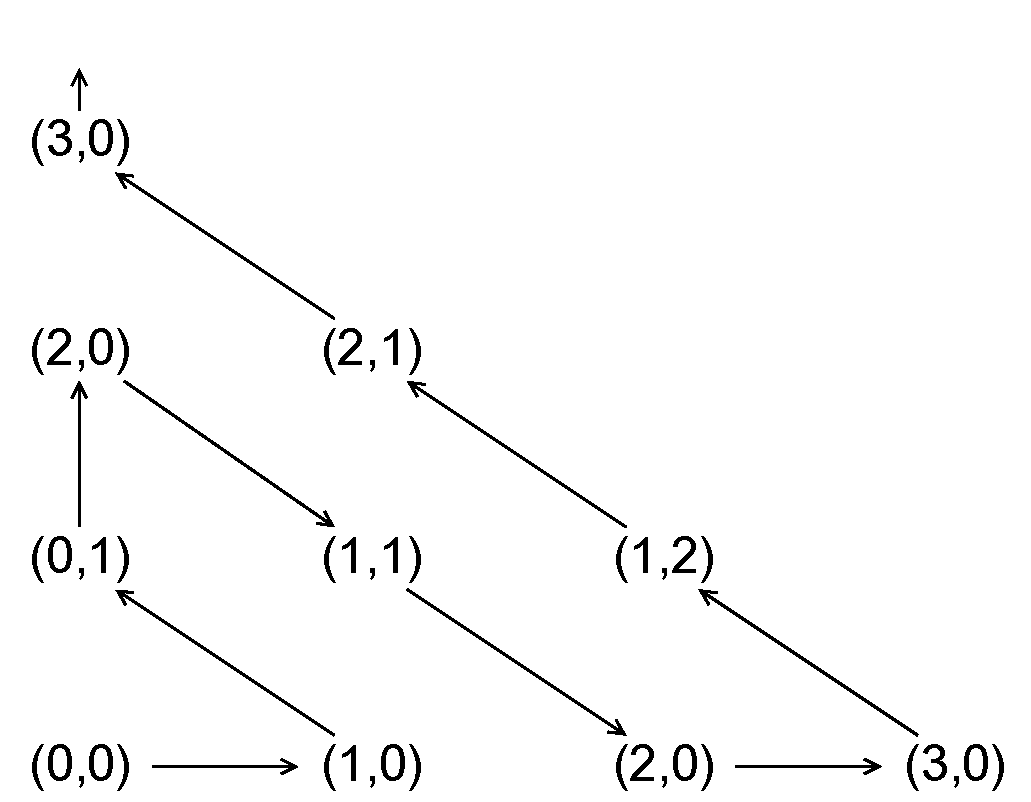
\includegraphics[width=0.5\linewidth]{images/figures/cantor1}
%\caption*{Die Pfeile deuten die Reihenfolge an, in der die Elemente von $\N\times\N$ abgezählt werden.}
\end{center}
\ %end{figure}
\end{proof}
\begin{satz}\label{satz:countableUnion}
Jede Vereinigung von abzählbar vielen abzählbaren Mengen ist abzählbar. Konkret, jede Vereinigung von der Form
\[
\bigcup_{i\in\N}A_i
\]
ist abzählbar, wenn alle $A_i$'s abzählbar sind.
\end{satz}
\begin{proof}
Wir nehmen an, dass die Menge $\{A_i\mid i\in \N \}$ aus lauter abzählbaren Mengen besteht. Um zu zeigen, dass $\bigcup_{i\in N}A_i$ abzählbar ist, genügt es, aufgrund von Satz~\ref{satz:abzaehlbarTransitiv} und Satz~\ref{cantor1}, zu zeigen, dass es eine surjektive Funktion
\[
H:\N\times\N\to\bigcup_{i\in N}A_i
\]
gibt. Da für jede natürliche Zahl $i$ die Menge $A_i$ abzählbar ist, gibt es für jede natürliche Zahl $i$ auch eine surjektive Funktion $F_i:\N\to A_i$. Wir können die Vereinigungsmenge der $A_i$'s also wie folgt schreiben:
\begin{align*}
\bigcup_{i\in \N}A_i&=\{F_i(j)\mid i,j\in\N \}\\
&=\{F_i(j)\mid (i,j)\in\N\times\N \}.
\end{align*}
Daraus folgt, dass die Funktion
\[
H:\N\times\N\to \bigcup_{i\in N}A_i\phantom{abstand}\text{mit}\phantom{abstand} H(i,j)=F_i(j),
\]
die gesuchte surjektive Funktion ist.
\end{proof}

\begin{cor}
Die Menge $\Z\times \Z$ ist abzählbar.
\end{cor}
\begin{proof}
Wir wissen bereits, dass die Menge $\N\times\N$ abzählbar ist. Daraus folgt, dass auch die Mengen
\begin{align*}
X&=\N\times\{-n\mid n\in \N\}\\
Y&=\{-n\mid n\in \N\}\times\N \\
Z&=\{-n\mid n\in \N\}\times\{-n\mid n\in \N\}
\end{align*}
abzählbar sind. Aus Satz~\ref{satz:countableUnion} folgt also, dass die Menge
\[
\Z\times\Z=(\N\times\N)\cup X\cup Y\cup Z
\]
abzählbar ist.
\end{proof}

\begin{cor}
Die Menge $\Q=\big\{\frac{x}{y}\mid x,y\in \Z\big\}$ der rationalen Zahlen (Brüche) ist abzählbar.
\end{cor}
\begin{proof}
Da die Funktion
\[
F:\Z\times(\Z\setminus{\{0\}})\to \Q\phantom{abstand}\text{mit}\phantom{abstand}F(x,y)=\frac{x}{y}
\]
surjektiv ist, folgt die Behauptung aus Satz~\ref{satz:abzaehlbarTransitiv}.
\end{proof}

\begin{ueb}
Ist die Menge aller endlichen Teilmengen von $\N$ abzählbar? Begründen Sie Ihre Antwort.
\end{ueb}
\begin{lsg}
\ifthenelse{\boolean{ml}}{
Wir können jede endliche Menge von natürlichen Zahlen mittels ihrer charakteristischen Funktion (vgl. Vorlesung) mit einer endlichen Binärsequenz identifizieren. Durch das Hinzufügen einer führenden $1$ zu jeder endlichen Binärsequenz entspricht jede dieser Sequenzen einer natürlichen Zahl in Binärdarstellung. Daraus folgt die Behauptung.}{~\answerspace{7cm}}
\end{lsg}

\begin{thrm}[Zweites Diagonalargument]\label{thrm:cantor2}
Die Menge aller unendlichen Binärsequenzen (Sequenzen aus Nullen und Einsen) ist überabzählbar.
\end{thrm}
\begin{proof}
Beweis durch Widerspruch. Wäre die Menge aller unendlichen Binärsequenzen abzählbar, dann gäbe es eine Liste von der Form\footnote{Natürlich ist die angedeutete Liste Beispielhaft und dient nur der Veranschaulichung unserer Konstruktion der Sequenz $b$. Die Sequenz $s_0$, beispielsweise, könnte auch mit dem Präfix $00000100$ oder irgend einer anderen Folge von Nullen und Einsen beginnen. }
\begin{center}
\begin{tabular}{c|l}
$\N$ & Binärsequenzen\\
\hline
$0$ & $s_0=01101011\cdots$\\
$1$ & $s_1=10010110\cdots$\\
$2$ & $s_2=00101001\cdots$\\
$\vdots$ & $\vdots$
\end{tabular}
\end{center}
in der alle unendlichen Binärsequenzen vorkommen. Wir konstruieren nun, ausgehend von dieser Liste, eine Binärsequenz $b$, die nicht in der Liste enthalten sein kann. Wir definieren $b$ wie folgt:
\begin{align*}
0\text{-tes Glied}&=b(0)=1-s_0(0)\\
1\text{-tes Glied}&=b(1)=1-s_1(1)\\
2\text{-tes Glied}&=b(2)=1-s_2(2)\\
&\vdots\\
n\text{-tes Glied}&=b(n)=1-s_n(n)\\
&\vdots
\end{align*}
Die Folge $b=110\cdots$ kann nicht in der Liste vorkommen, weil sie sich von jedem Element in der Liste in mindestens einem Glied unterscheidet (von der $n$-ten Sequenz unterscheidet sich $b$ im $n$-ten Glied). Dies steht im Widerspruch zu unserer Annahme, dass in der Liste alle unendlichen Binärsequenzen vorkommen.
\end{proof}


\begin{cor}
Das Intervall $(0,1)=\{r\in\R\mid 0<r<1 \}$ ist überabzählbar. Insbesondere ist die Menge $\R$ der reellen Zahlen überabzählbar.
\end{cor}
\begin{proof}
Die reellen Zahlen (in Binärdarstellung) im Intervall $(0,1)$, sind von der Form $0,\dots$ wobei $\dots$ für eine unendliche Binärsequenz steht. Daher steht das Intervall $(0,1)$ mit der Menge aller unendlichen Binärsequenzen in eins-zu-eins Korrespondenz. Die Behauptung folgt daher aus Theorem~\ref{thrm:cantor2}.
\end{proof}

\begin{cor}
Die Potenzmenge von $\N$ ist überabzählbar.
\end{cor}
\begin{proof}
Jede Teilmenge $A$ von $\N$ kann wie folgt durch eine Binärsequenz $\chi_A$ beschrieben werden:
\begin{align*}
\chi_A(n)=\begin{cases}
1&\text{falls } n\in A\\
0&\text{falls} n\notin A.
\end{cases}
\end{align*}
Daher folgt die Behauptung aus Theorem~\ref{thrm:cantor2}.
\end{proof}

\begin{cor}
Die Menge aller Funktionen $F:\N\to\N$ ist überabzählbar.
\end{cor}
\begin{proof}
Die Menge der Binärsequenzen entspricht der Menge der Funktionen $F:\N\to\{0,1\}$. Daher folgt die Behauptung aus Theorem~\ref{thrm:cantor2}.
\end{proof}

\begin{cor}
Es gibt Funktionen $F:\N\to\N$, die von keinem Java, C, C++, Fortran\dots Programm berechenbar sind. Solche Funktionen heissen \textit{unberechenbar}.
\end{cor}


\begin{ueb}
Zeigen Sie, dass die Menge
\[
U=\{1,11,111,1111,\dots \}
\]
aller endlichen Sequenzen von Einsen abzählbar ist. Ist die Menge aller (abzählbar) unendlichen Sequenzen von Einsen auch abzählbar?
\end{ueb}
\begin{lsg}
\ifthenelse{\boolean{ml}}{
	Wir müssen zeigen, dass eine surjektive Abbildung $F:\N\to \{1,11,\dots\}$ existiert. Da dies z.B. für die Funktion
	\begin{align*}
	F(n)=\underbrace{11\dots 1}_{n\text{ viele}}
	\end{align*}
	erfüllt ist, gilt die Behauptung. Die Menge aller (abzählbar) unendlichen $1$-Sequenzen besteht aus nur einem Element und ist somit natürlich abzählbar. }
{~\answerspace{2cm}}
\end{lsg}

\subsection{Ordnungs- und Äquivalenzrelationen}

Neben den Funktionen und ihren Anwendungen gibt es in der Mathematik noch zahlreiche weitere wichtige Klassen von Relationen. Im Folgenden wollen wir auch aufgrund ihrer Wichtigkeit in der Informatik die Ordnungsrelationen (inklusive Halbordnungen) und Äquivalenzrelationen etwas genauer betrachten. Wie viele Typen von Relationen werden auch Ordnungen und Äquivalenzen aufgrund von bestimmten Kombinationen von Grundeigenschaften definiert. Folgend einige wichtige solche Grundeigenschaften.


\begin{df}
    Eine binäre Relation $R$ auf einer Menge $X$ heisst:
    \begin{itemize}
    \item \textit{Reflexiv}, wenn für alle $x\in X$
    \[
    xRx
    \]
    gilt.
    \item \textit{Symmetrisch}, wenn für alle $x,y\in X$
    \[
    xRy\,\Rightarrow\, yRx
    \]
    gilt.
    \item \textit{Antisymmetrisch}, wenn für alle $x,y\in X$
    \[
    xRy\land yRx\,\Rightarrow x=y
    \]
    gilt.
    \item \textit{Transitiv}, wenn für alle $x,y,z\in X$
    \[
    xRy\land yRz\,\Rightarrow \, xRz
    \]
    gilt.
    \end{itemize}
    \end{df}


    \begin{rk}
    Die Relation $R\subseteq X\times X$ ist genau dann reflexiv, wenn die Diagonale
    \[
    \Delta_X:=\{(x,x)\mid x\in X \}
    \]
    eine Teilmenge von $R$ ist. Grafisch heisst das, dass die Diagonale (rot markiert) in $R$ enthalten ist.
    \begin{center}
    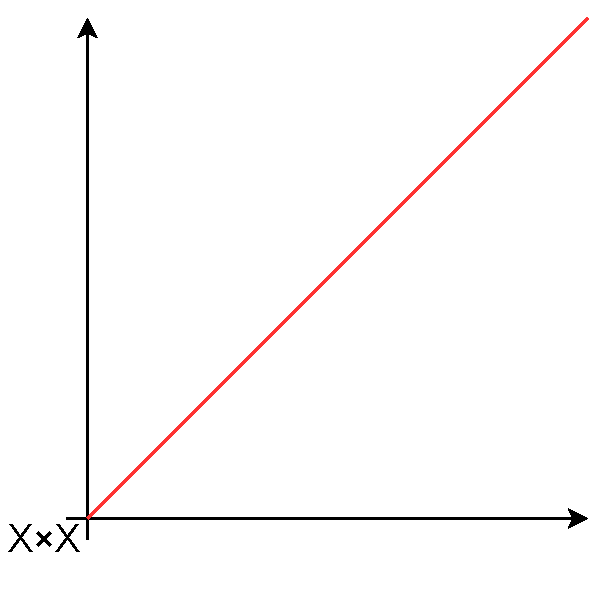
\includegraphics[width=0.2\linewidth]{images/figures/diagonale}
    \end{center}
    Die Relation $R$ ist symmetrisch, wenn ihr Graph symmetrisch bezüglich der Geraden $\Delta_X$ ist.
    \end{rk}


    \begin{bsp}
        Wir betrachten nochmals die Verliebtheitsrelation aus Beispiel \ref{ex:Beispiel1relationen}:
        \[
        pLq:\Leftrightarrow \text{Person $p$ liebt Person $q$.}
        \]
    Die Verliebtheitsrelation hat unter anderem folgende Eigenschaften:
    \begin{itemize}
        \item $L$ ist nicht reflexiv, da nicht alle Menschen ``selbstverliebt'' sind.
        \item $L$ ist (leider\footnote{Andererseits gäbe es wohl keine Literatur oder gar Kunst, wenn diese Relation tatsächlich symmetrisch wäre.}) nicht symmetrisch, da Liebe nicht immer auf Gegenseitigkeit beruht.
        \item $L$ ist nicht Antisymmetrisch, da es durchaus ``echte'' Liebespaare (aus zwei Partnern bestehend) gibt.
        \item $L$ ist nicht transitiv, da die meisten Leute den angebeteten der eigenen angebeteten nicht lieben (ganz im Gegenteil!).
    \end{itemize}
    \end{bsp}

    \begin{ueb}
        Geben Sie binäre Relationen (auf der Menge aller Menschen) mit folgenden Eigenschaften an:
        \begin{enumerate}
            \item Transitiv und nicht antisymmetrisch.
            \item Transitiv, reflexiv und antisymmetrisch.
            \item Nicht reflexiv, nicht transitiv.
        \end{enumerate}
    \end{ueb}
    \begin{lsg}
        \ifthenelse{\boolean{ml}}{
            Zum Beispiel:
            \begin{enumerate}
                \item $pJq:\Leftrightarrow $ Person $p$ ist jünger oder gleichalt (in Jahren) wie Person $q$.
                \item $pWq:\Leftrightarrow$ Person $p$ ist echt jünger als Person $q$.
                \item $pGq:\Leftrightarrow$ Person $p$ ist vom anderen Geschlecht als Person $q$.
            \end{enumerate}
            }{~
            \answerspace{5cm}
            }
    \end{lsg}


    \subsection*{Äquivalenzrelationen}

    Äquivalenzrelationen sind in einem gewissen Sinn (konkret im Sinn von Satz~\ref{satz: equivalenzen verallgemeinerte gleichheit}) verallgemeinerte Gleichheitsrelationen. Sie werden dazu verwendet, (im Sinn der Relation) ähnliche Objekte miteinander zu identifizieren und als ``gleich'' zu behandeln.

    \begin{df}
    \textit{Äquivalenzrelationen} sind reflexive, symmetrische und transitive Relationen.
    \end{df}

    \begin{bsp}
    Auf jeder Menge $X$ ist die Gleichheitsrelation $\Delta_X=\{(x,x)\mid x\in X \}$ eine Äquivalenzrelation. Weil jede Äquivalenzrelation reflexiv ist, ist die Gleichheitsrelation auf jeder Menge die ``kleinste'' Äquivalenzrelation. Am anderen Ende des Spektrums steht die Relation $X\times X$, sie ist die grösste Äquivalenzrelation auf der Menge $X$.
    \end{bsp}

    \begin{bsp}
    Von den Relationen $R_1,R_2,R_3$ und $T$ aus Beispiel~\ref{ex:Beispiel1relationen}, sind $R_1,R_2$ Äquivalenzrelationen.
    \begin{itemize}
    \item Die Relation $R_3$ ist keine Äquivalenzrelation, weil sie nicht reflexiv (nicht jeder liebt sich selbst), nicht symmetrisch (es gibt unglücklich Verliebte) und nicht transitiv ist. Man beachte, dass jeder einzelne der genannten Gründe genügt, damit $R_3$ keine Äquivalenzrelation ist.
    \item Die Relation $T$ ist zwar reflexiv und transitiv, aber nicht symmetrisch und daher auch keine Äquivalenzrelation.
    \end{itemize}
    \end{bsp}


    \begin{df}
    Es sei $R$ eine Äquivalenzrelation auf einer Menge $X$ und $x\in X$. Die \textit{Äquivalenzklasse} $[x]_R$ von $x$ bezüglich $R$ ist die Menge aller Elemente von $X$, die zu $x$ in Relation $R$ stehen:
    \[
    [x]_R:=\{y\in X\mid xRy \}
    \]
    Jedes Element einer Äquivalenzklasse nennen wir einen \textit{Repräsentanten} der entsprechenden Äquivalenzklasse. Die \textit{Faktormenge} $\faktor{X}{R}$ \textit{von} $X$ \textit{modulo} $R$ ist die Menge aller Äquivalenzklassen:
    \[
    \faktor{X}{R}:=\big\{ [x]_R\mid x\in X \big\}
    \]
    \end{df}

    \begin{bsp}\label{bsp:modulo5relation}
    Wir betrachten die Relation $\equiv_5$ auf der Menge $\Z$, die wie folgt gegeben ist:
    \[
    x\equiv_5 y:\Leftrightarrow (x-y)\text{ ist ein Vielfaches von  }5.
    \]
    Als Java Code könnte man die Relation auch wie folgt darstellen:

    \begin{framed}
        \begin{lstlisting}{static,boolean}
    static boolean Rel(int x, int y){
        if (y<0) return Rel(x,y+5);
        if (x<0) return Rel(x+5,y);
        if (y>=5) return Rel(x,y-5);
        if (x>=5) return Rel(x-5,y);
        return x == y;
    }
    \end{lstlisting}
    \end{framed}
    Wir überzeugen uns nun davon, dass diese Relation eine Äquivalenzrelation ist.
    \begin{itemize}
    \item \textbf{Reflexivität}: Es gilt für jede ganze Zahl $z$
    \[
    0\cdot 5=0=(z-z).
    \]
    Also ist $(z-z)$ ein Vielfaches von $5$, somit gilt $z\equiv_5 z$.
    \item\textbf{Symmetrie}: Gilt $x\equiv_5 y$, dann gibt es eine ganze Zahl $z$ mit $5z=(x-y)$. Also ist auch
    \[
    (y-x)=-(x-y)=-5z=5\cdot(-z)
    \]
    ein Vielfaches von $5$, d.h. es gilt $y\equiv_5x$.
    \item\textbf{Transitivität}: Gilt $x\equiv_5 y$ und $y\equiv_5 z$, dann gibt es ganze Zahlen $r,s$ mit $5r=x-y$ und $5s=y-z$. Insgesamt erhalten wir, dass
    \[
    x-z=(x-y)+(y-z)=5r+5s=5(r+s)
    \]
    ein Vielfaches von $5$ ist und somit, dass $x\equiv_5 z$ gilt.
    \end{itemize}
    Wir betrachten nun die Äquivalenzklassen modulo der Relation $\equiv_5$ (diese heissen Restklassen modulo $5$).
    \begin{align*}
    [0]_{\equiv_5}&=\{x\in \Z\mid 0\equiv_5y \}\\ &=\{z\in\Z\mid z\text{ ist ein Vielfaches von }5 \}\\
    &=\{5z\mid z\in\Z \}\\
    \phantom{dd}\\
    [1]_{\equiv_5}&=\{x\in \Z\mid 1\equiv_5y \}\\ &=\{z\in\Z\mid \text{ Bei Division durch }5\text{ lässt }z\text{ den Rest }1 \}\\
    &=\{5z+1\mid z\in\Z\}\\
    \phantom{dd}\\
    [2]_{\equiv_5}&=\{x\in \Z\mid 2\equiv_5y \}\\ &=\{z\in\Z\mid \text{ Bei Division durch }5\text{ lässt }z\text{ den Rest }2 \}\\
    &=\{5z+2\mid z\in\Z\}\\
    \phantom{dd}\\
    [3]_{\equiv_5}&=\{x\in \Z\mid 3\equiv_5y \}\\ &=\{z\in\Z\mid \text{ Bei Division durch }5\text{ lässt }z\text{ den Rest }3 \}\\
    &=\{5z+3\mid z\in\Z\}\\
    \phantom{dd}\\
    [4]_{\equiv_5}&=\{x\in \Z\mid 4\equiv_5y \}\\ &=\{z\in\Z\mid \text{ Bei Division durch }5\text{ lässt }z\text{ den Rest }4 \}\\
    &=\{5z+4\mid z\in\Z\}
    \end{align*}
    Die Faktormenge der Relation $\equiv_5$ ist also durch
    \[
    \faktor{\Z}{\equiv_5}=\{ [0]_{\equiv_5},[1]_{\equiv_5},[2]_{\equiv_5},[3]_{\equiv_5},[4]_{\equiv_5} \}
    \]
    gegeben.
    \end{bsp}
    \begin{lm}\label{lm:sim gleiche klasse}
    Ist $\sim $ eine Äquivalenzrelation auf einer Menge $X$ und gilt $x,y\in X$ mit $x\sim y$, dann gilt $[x]_\sim=[y]_\sim$. Mit anderen Worten, äquivalente Elemente repräsentieren stets dieselbe Äquivalenzklasse.
    \end{lm}
    \begin{proof}
    Seien $X,\sim,x,y$ wie in der Behauptung. Um zu zeigen, dass $[x]_\sim=[y]_\sim$ gilt, genügt es nachzuweisen, dass $x\sim z\Leftrightarrow y\sim z$ für beliebige $z\in X$ gilt. Wir nehmen $x\sim y$ an, dann gilt
    \begin{align*}
    y\sim z\Rightarrow x\sim y\land y\sim z \stackrel{\text{Transitivität}}{\Longrightarrow} x\sim z
    \end{align*}
    und
    \[
    x\sim z\Rightarrow x\sim y\land x\sim z\stackrel{\text{Symmetrie}}{\Longrightarrow} y\sim x\land x\sim z\stackrel{\text{Transitivität}}{\Longrightarrow} y\sim z,
    \]
    wie gewünscht.
    \end{proof}
    \begin{cor}\label{cor:alle Elemente Repräsentanten}
    Ist $\sim $ eine Äquivalenzrelation auf $X$ und sind $x,y\in X$ mit $x\in[y]_\sim$, dann gilt $[x]_\sim=[y]_\sim$. Mit anderen Worten, jedes Element einer Äquivalenzklasse ist auch ein Repräsentant dieser Äquivalenzklasse.
    \end{cor}
    \begin{proof}
    Es seien $X,\sim,x$ und $y$ wie in der Behauptung. Aus $x\in[y]_\sim$ folgt $y\sim x$. Die Behauptung folgt nun aus Lemma~\ref{lm:sim gleiche klasse}.
    \end{proof}

    \begin{satz}\label{satz: equivalenzklassen disjunkt}
    Ist $\sim $ eine Äquivalenzrelation auf $X$ und sind $x,y\in X$ mit $[x]_\sim\neq[y]_\sim$, dann gilt $[x]_\sim\cap[y]_\sim=\varnothing$.
    Mit anderen Worten, verschiedene Äquivalenzklassen sind immer disjunkt.
    \end{satz}
    \begin{proof}
    Es seien $X,\sim,x$ und $y$ wie in der Behauptung. Wir zeigen die Kontraposition, d.h.
    \[
    [x]_\sim\cap[y]_\sim\neq\varnothing\Rightarrow [x]_\sim=[y]_\sim.
    \]
    Es gelte also $[x]_\sim\cap[y]_\sim\neq\varnothing$, es gibt daher ein $z\in [x]_\sim\cap[y]_\sim$. Daraus folgt, dass $x\sim z\land y\sim z$ gilt und wegen der Transitivität und der Symmetrie von $\sim$ folgt sofort $x\sim y$. Die Behauptung folgt nun aus Lemma~\ref{lm:sim gleiche klasse}.
    \end{proof}


    \begin{satz}\label{satz: equivalenzklassen partition}
    Ist $\sim$ eine Äquivalenzrelation auf einer Menge $X$, dann ist die Faktormenge $\faktor{X}{\sim}$ eine Partition von $X$.
    \end{satz}
    \begin{proof}
    Es sei $\sim$ eine beliebige Äquivalenzrelation auf einer Menge $X$. Wir müssen folgende Punkte verifizieren:
    \begin{enumerate}
    \item\label{a} Die Äquivalenzklassen sind alle nichtleer.
    \item\label{2} Die Äquivalenzklassen sind paarweise disjunkt.
    \item\label{3} Es gilt
    \[
    \bigcup_{x\in X}[x]_{\sim}=X.
    \]
    \end{enumerate}
    Der erste Punkt folgt aus der Definition von der Faktormenge (die Äquivalenzklassen sind via ihrer Repräsentanten definiert). Die Tatsache, dass die Äquivalenzklassen paarweise disjunkt sind, ist genau die Aussage von Satz~\ref{satz: equivalenzklassen disjunkt}. Wir brauchen also bloss noch den letzten Punkt zu verifizieren. Dies folgt, da für jedes $z\in X$, wegen der Reflexivität, $z\sim z$ und somit
    \[
    z\in[z]_\sim\subseteq\bigcup_{x\in X}[x]_\sim
    \]
    gilt.
    \end{proof}

    \begin{rk}
        Das Konzept von Äquivalenzklassen (und deren Zusammenhang mit Partitionen) werden Sie in der theoretischen Informatik in Form von sogenannten ``Zustandsklassen'' wiederfinden, diese werden dort gebraucht, um zu zeigen, dass es Sprachen gibt, die nicht mit ``endlichen Zustandsautomaten'' erkannt werden können.
    \end{rk}

    \begin{ueb}\label{greg}
        Gegeben Sei die Äquivalenzrelation
        \[
            pRq:\Leftrightarrow\text{$p$ hat am gleichen Tag Geburtstag wie $q$.}
        \]
        Kommentieren Sie folgende Aussagen mit ``wahr'', ``falsch'' oder ``unklar'' unter der
        Annahme $Ray\, R\, Greg $:
        \begin{enumerate}
            \item Ray ist älter als Greg oder Greg ist älter als Ray.
            \item Ray und Greg sind gleich alt.
            \item Ray ist verwandt mit Greg.
            \item Der Altersunterschied von Ray und Greg in Jahren ist ganzzahlig.
        \end{enumerate}
    \end{ueb}
    \begin{lsg}
        \ifthenelse{\boolean{ml}}{
            $d)$ ist wahr, die restlichen Aussagen sind aufgrund der Annahmen nicht entscheidbar.}
            {~
                \answerspace{2cm}}
    \end{lsg}

    \begin{ueb}
        Wie viele Äquivalenzklassen hat die Relation $R$ von Übung \ref{greg}?
    \end{ueb}
    \begin{lsg}
        \ifthenelse{\boolean{ml}}{
            $366$ (Auch in Schaltjahren haben an jedem Tag Leute Geburtstag.)}{~
            \answerspace{1cm}}
    \end{lsg}

    Wir haben in Satz~\ref{satz: equivalenzklassen partition} gesehen, dass jede 	Äquivalenzrelation auf einer Menge eine Partition auf eben dieser Menge induziert. Als Nächstes sehen wir, dass auch die Umkehrung gilt; jede Partition induziert eine Äquivalenzrelation, deren Faktormenge genau der ursprünglichen Partition entspricht. Insgesamt sehen wir, dass eine eins-zu-eins Korrespondenz zwischen allen möglichen Partitionen und allen möglichen Äquivalenzrelationen auf einer gegebenen Menge existiert.

    \begin{satz}
    Ist $P=\{A_i\mid i\in I\}$ eine Partition von der Menge $X$, dann ist die Relation $\sim$, gegeben durch
    \[
    x\sim y:\Leftrightarrow \exists i\in I\,(x\in A_i\land y\in A_i),
    \]
    eine Äquivalenzrelation auf $X$. Zusätzlich gilt
    \[
    \faktor{X}{\sim}=P.
    \]
    \end{satz}
    \begin{proof}
    Zuerst zeigen wir, dass die Relation $\sim$ unter den gegebenen Umständen eine Äquivalenzrelation ist.
    \begin{itemize}
    \item \textbf{Reflexivität}: Sei $x\in X$  beliebig. Wir müssen zeigen, dass $x\sim x$ gilt. Da $P=\{A_i\mid i\in I\}$ eine Partition von $X$ ist, gibt es ein $i\in I$ mit $x\in A_i$, daraus folgt sofort $x\sim x$.
    \item \textbf{Symmetrie}: Es gelte $x\sim y$. Wir müssen $y\sim x$ zeigen. Aus $x\sim y$ folgt, dass es ein $i\in I$ mit $x\in A_i\land y\in A_i$ gibt, dies ist offensichtlich äquivalent zu $y\sim x$.
    \item \textbf{Transitivität}: Es gelte $x\sim y\land y\sim z$. Wir müssen $x\sim z$ zeigen. Aus $x\sim y\land y\sim z$ folgt, dass es $i,j\in I$ gibt so, dass $x,y\in A_i$ und $y,z\in A_j$ gilt. Da $P=\{A_i\mid i\in I\}$ eine Partition ist, kann $y $ nicht in zwei verschiedenen Blöcken enthalten sein, es gilt daher $i=j$ und somit $x\sim z$.
    \end{itemize}
    Dass die Äquivalenzklassen von $\sim$ genau den Blöcken von $P$ entsprechen ist sofort klar, wenn man beachtet, dass zwei Elemente genau dann äquivalent sind, wenn sie im selben Block von $P$ liegen.
    \end{proof}

    Am Anfang dieses Abschnittes haben wir Äquivalenzrelationen als verallgemeinerte Gleichheitsrelationen beschrieben, dies können wir im folgenden Satz präzisieren.

    \begin{satz}\label{satz: equivalenzen verallgemeinerte gleichheit}
    Für jede Relation $\sim$ auf einer Menge $X$ sind folgende beiden Aussagen äquivalent.
    \begin{enumerate}
    \item[1.] Die Relation $\sim$ ist eine Äquivalenzrelation.
    \item[2.] Es gibt eine Menge $Y$ und ein Funktion $F:X\to Y$ so, dass für alle $x,y\in X$
    \[
    x\sim y\Leftrightarrow F(x)=F(y)
    \]
    gilt.
    \end{enumerate}
    \end{satz}
    \begin{proof}
    Wenn $\sim$ eine Äquivalenzrelation auf der Menge $X$ ist, dann erfüllt die Abbildung
    \[
    F:X\to\mathcal{P}(X)\phantom{abstand}\text{mit} \phantom{abstand} F(x)=[x]_\sim
    \]
    alle geforderten Eigenschaften. Ist umgekehrt eine Funktion $F:X\to Y$ wie in der Behauptung gegeben, dann gilt für die Relation $\sim$ Folgendes:
    \begin{itemize}
    \item\textbf{Reflexivität} gilt, da für jedes Element $x\in X$ trivialerweise $F(x)=F(x)$ gilt.
    \item \textbf{Symmetrie} folgt, da für beliebige Elemente $x,y\in X$
    \[
    x\sim y\Rightarrow F(x)=F(y)\Rightarrow F(y)=F(x)\Rightarrow y\sim x
    \]
    gilt.
    \item\textbf{Transitivität} folgt, da für beliebige Elemente $x,y,z\in X$
    \[
    x\sim y\land y\sim z\Rightarrow F(x)=F(y)\land F(y)=F(z)\Rightarrow F(x)=F(z)\Rightarrow  x\sim z
    \]
    gilt.
    \end{itemize}
    \end{proof}



    \begin{bsp}
    Es sei $\sim_{14}$ die folgendermassen auf der Menge $Fun(\R)=\{F\mid F:\R\to\R\}$ gegebene Relation:
    \[
    F\sim G:\Leftrightarrow F(14)=G(14).
    \]
    Wir betrachten die Funktion
    \[
    Eval_{14}:Fun(\R)\to \R\phantom{abstand}\text{mit}\phantom{abstand}Eval_{14}(F)=F(14).
    \]
    Offenbar gilt
    \[
    F\sim_{14}G\Leftrightarrow Eval_{14}(F)=Eval_{14}(G).
    \]
    Anhand von Satz~\ref{satz: equivalenzen verallgemeinerte gleichheit} sehen wir also sofort, dass es sich bei $\sim_{14}$ um eine Äquivalenzrelation handelt.
    \end{bsp}

    \begin{rk}[Wohldefiniertheitsproblem]
    Wir betrachten die Relation $\simeq$, die auf der Menge $\N$ folgendermassen gegeben ist.
    \[
    n\simeq m\Leftrightarrow n,m\text{ haben die gleichen Primteiler}.
    \]
    Nun definieren wir eine Funktion
    \[
    F:\faktor{\N}{\simeq}\to \N\phantom{abstand}F([x]_\simeq):=x+102.
    \]
    Es soll zum Beispiel $F([7]_\simeq)=109$ gelten. Sehen Sie ein Problem bei unserem Vorgehen? Ist $F([49]_\simeq)=151$? Es gilt doch $7\simeq 49$ und somit auch $[7]_\simeq=[49]_\simeq$. Sollte dann nicht auch $F([7]_\simeq)=F([49]_\simeq)$ gelten? Natürlich schon! Das Problem, das wir hier haben, nennt man ein \textit{Wohldefiniertheitsproblem}. Es entsteht, wenn man Funktionswerte von Äquivalenzklassen mit Bezugnahme auf deren Repräsentanten definiert, ohne sicherzustellen, dass der Funktionswert nicht von der Wahl der Repräsentanten abhängt.

    Sind eine Äquivalenzrelation $\sim$ auf einer Menge $X$ und eine Funktion $F:X\to Y$ gegeben, so erhält man nur dann durch die Zuordnung
    \[
    \tilde F([x]_\sim):=F(x)
    \]
    eine wohldefinierte Funktion
    \[
    \tilde F:\faktor{X}{\sim}\to Y,
    \]
    wenn die Funktion $F$ mit der Relation $\sim$ verträglich ist. Das heisst, wenn
    \[
    x\sim y\Rightarrow F(x)=F(y)
    \]
    gilt.
    \end{rk}

    \begin{bsp}
    Ein Beispiel (vgl.~\ref{bsp:modulo5relation}) für eine wohldefinierte Abbildung
    \[
    F:\faktor{\Z}{\equiv_5}\to\faktor{\Z}{\equiv_5}
    \]
    erhalten wir z.B. durch die Zuordnung
    \[
    F([x]_{\equiv_5}):=[2x+3]_{\equiv_5}.
    \]
    Um zu sehen, dass diese Funktion tatsächlich wohldefiniert ist, betrachten wir:
    \begin{align*}
    x\equiv_5 y&\Rightarrow (x-y)\text{ ist Vielfaches von } 5\\
    &\Rightarrow\exists z\in\Z\,(5z=x-y)\\
    &\Rightarrow \exists z\in\Z\,\big((2x+3)-(2y+3)=2x-2y=2(x-y)=5(2z)\big)\\
    &\Rightarrow (2x+3)-(2y+3)\text{ ist ein Vielfaches von }5\\
    &\Rightarrow [2x+3]_{\equiv_5}=[2y+3]_{\equiv_5}\\
    \end{align*}
    \end{bsp}


    \subsection*{Ordnungsrelationen}

    Unter Ordnungsrelationen fasst man alle Arten von Relationen zusammen, mithilfe derer man
    Objekte in gewisser Weise vergleichen und mehr oder weniger eindeutig sortieren kann. Das
    Standardbeispiel ist die Ordnungsrelationen $\leq$ auf den verschiedenen Zahlenmengen.

    \begin{df}\label{df:minimale elemente}
    Es sei $R$ eine binäre Relation auf der Menge $M$.
    \begin{itemize}
    \item Zwei Elemente $x,y\in M$ heissen $R$-\textit{unvergleichbar}, falls weder $xRy$ noch $yRx$ gilt.
    \item Ein Element $x\in X$ einer Teilmenge $X\subseteq M$ von $M$ heisst $R$-\textit{minimal in $X$}, falls es kein anderes Element $y\in X$ mit $yRx$ gibt.
    \item  Ein Element $x\in X$ einer Teilmenge $X\subseteq M$ von $M$ heisst $R$-\textit{maximal in $X$}, falls es kein anderes Element $y\in X$ mit $xRy$ gibt.
    \end{itemize}
    Wenn keine Missverständnisse zu befürchten sind, dann schreiben wir anstelle von $R$-minimal, $R$-maximal und $R$-unvergleichbar auch einfach minimal, maximal und unvergleichbar.
    \end{df}

    \begin{ueb}
        Es sei $R$ die Gleichheitsrelation auf der Menge der natürlichen Zahlen. Welches sind die $R$-minimalen und $R$-maximalen Elemente?
    \end{ueb}
    \begin{lsg}~
        \ifthenelse{\boolean{ml}}{
            Alle natürlichen Zahlen sind sowohl minimal als auch maximal bezüglich der Gleichheitsrelation.
            }{~
            \answerspace{0cm}
            }
    \end{lsg}

    \begin{rk}
        Es sei $X$ eine Teilmenge von $M$ und $R$ eine binäre Relation auf $M$.
        Die $R$-minimalen Elemente von $X$ entsprechen im Graph $G=(M,R)$ genau den Knoten, bei
        denen keine Pfeile enden, die ihren Ursprung in $X$ haben. Die maximalen Elemente
        entsprechen den Knoten, von denen alle ausgehenden Pfeile aus der Menge $X$
        ``hinauszeigen''. Zwei Elemente $x,y\in M$ sind $R$-unvergleichlich, wenn es keine
        Pfeile (egal in welcher Richtung) gibt, die $x$ und $y$ verbinden.
    \end{rk}

    \begin{ueb}
    Die Relation $R$ auf der Menge $M=\{a,b,u,v,x,y,z\}$ sei durch den Graph $(M,R)$ wie folgt
    gegeben.
    \begin{center}
    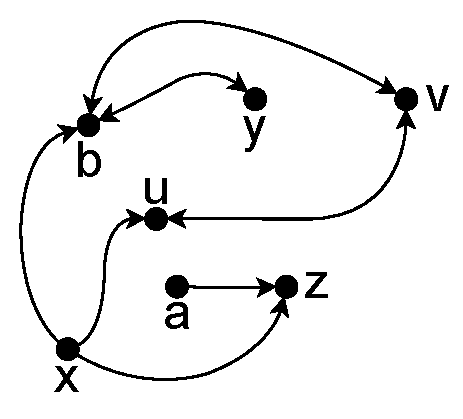
\includegraphics[width=0.5\linewidth]{images/graphviz/maxmingraph}
    \end{center}
    Geben Sie alle minimalen und maximalen Elemente von $M$ an. Geben Sie weiter zwei Elemente an, die unvergleichbar sind.
    \end{ueb}
    \begin{lsg}~
    \ifthenelse{\boolean{ml}}{
        \begin{itemize}
            \item Die minimalen Elemente von $M$ sind $a$ und $x$.
            \item Das einzige maximale Elemente von $M$ ist $z$.
            \item Die Elemente $a$ und $x$ sind z.B. unvergleichbar.
        \end{itemize}
        }{~
        \answerspace{4cm}}
    \end{lsg}

    \begin{df}
    Es sei $R$ eine binäre Relation auf der Menge $M$.
    \begin{itemize}
    \item $R$ ist eine \textit{Präordnung} auf $M$, wenn $R$ reflexiv und transitiv ist.
    \item $R$ ist eine \textit{Halbordnung} auf $M$, wenn $R$ reflexiv, antisymmetrisch und transitiv ist.
    \item $R$ ist eine \textit{totale oder lineare Ordnung} auf $M$, wenn $R$ eine Halbordnung ist und keine $R$-unvergleichbaren Elemente existieren.
    \item $R$ ist eine \textit{Wohlordnung} auf $M$, wenn $R$ eine totale Ordnung auf $M$ ist so, dass jede Teilmenge $X\neq\varnothing$ von $M$ (mindestens) ein $R$-minimales Element enthält.
    \end{itemize}
    \end{df}


    \begin{bsp}~
    \begin{itemize}
    \item Die Relation $\leq$ auf der Menge $\R$ ist eine totale Ordnung, die aber keine Wohlordnung ist (die Menge $\{x\in\R\mid 0<x<1\}$ hat kein kleinstes Element). Auf der Menge $\N$ ist $\leq$ eine Wohlordnung\footnote{Ein Beweis dazu kommt im nächsten Kapitel.}. Auf der Menge $\Z$ ist die Relation $\leq$ keine Wohlordnung. Wieso?
    \item Ist $A$ eine Menge von Mengen, dann ist die Teilmengenrelation $\subseteq$ eine Halbordnung.
    \item Die Teilerrelation $T$ auf der Menge $\Z$ ist eine Halbordnung aber keine totale Ordnung. Die Elemente $7$ und $5$ sind $T$-unvergleichlich.
    \end{itemize}
    \end{bsp}

    \begin{df}
        Es sei $R$ eine (bin\"are) Relation.
        \begin{itemize}
            \item Als \textit{transitiven Abschluss} von $R$ bezeichnet man die kleinste
            (bezüglich $\subseteq$) transitive Relation, die $R$ als Teilmenge enthält,
            sie wird mit $R^+$ notiert.
            \item Die kleinste Relation, die $R^+$ enthält und reflexiv ist, nennt man den
            \textit{reflexiv-transitiven Abschluss} von $R$, sie wird mit $R^*$ bezeichnet.
        \end{itemize}
    \end{df}

    \begin{rk}
        F\"ur eine beliebige (bin\"are) Relation $R$ gilt genau dann $xR^*y$, wenn es
        eine endliche Folge $x=k_1,\dots,k_n=y$ gibt, so dass $k_iRk_{i+1}$ f\"ur alle
        Indices $i=1,\dots,n-1$ gilt. Es gilt also genau dann $xR^*y$, wenn es eine Folge von
        Elementen gibt, die mit $x$ beginnt, mit $y$ endet und deren Elemente alle der Reihe
        nach in Relation $R$ zueinander stehen. Ist $G=(V,E)$ ein Graph, dann bedeutet
        $xE^*y$, dass in $G$ ein Pfad von $x$ nach $y$ existiert.
    \end{rk}

    \begin{df}
        Ein \textit{Weg} oder \textit{Pfad} in einem Graph $G=(V,E)$ ist eine endliche Folge
        $k_1,\dots,k_n\in V$ von Knoten, so dass $k_iEk_{i+1}$ f\"ur alle Indices
        $i=1,\dots,n-1$ gilt. Die Knoten $k_1$ und $k_n$ bezeichnet man als \textit{Anfangs-}
        und \textit{Endpunkt} des Pfades. Gilt zusätzlich $k_1=k_n$, dann spricht man von einem \textit{Zyklus}.
    \end{df}


    \begin{rk}
        In der Informatik wichtige Datenstrukturen sind sogenannte \textit{DAGs} (von ``directed acyclic graph''), gerichtete zyklenfreie Graphen. Eine der charakteristischen Eigenschaften von DAG's ist die Tatsache, dass sich ihre Elemente auf eine mit der Struktur des Graphen verträgliche Art sortieren lassen. Oft werden Abhängigkeiten von einzelnen Arbeitsschritten eines Prozesses als DAG modelliert, eine mit der Struktur des Graphen verträgliche lineare Ordnung der Knoten entspricht dann einer möglichen Reihenfolge in der die einzelnen Arbeitsschritte abgearbeitet werden können (ohne Abhängigkeiten zu verletzen).
    \end{rk}


    \begin{df}
        Es sei $M$ eine endliche Menge und $G=(M,E)$ ein DAG. Eine lineare Ordnung $\preceq\subseteq M\times M$ ist eine \textit{topologische Sortierung} von $G$, wenn für alle $a,b\in M$
        \begin{align*}
        a E^* b  \Rightarrow a\preceq b
        \end{align*}
        gilt.
    \end{df}

    \begin{satz}~
        Jeder endliche DAG besitzt (mindestens) eine topologische Sortierung.
    \end{satz}
    \begin{proof}
        Wir bemerken zuerst, dass jeder endliche DAG $G=(V,E)$ minimale Elemente bezüglich der Relation $E$ besitzt (wieso?). Weiter bemerken wir, dass jeder DAG, von dem ein minimaler Knoten (zusammen mit den von diesem Knoten ausgehenden Pfeilen) entfernt wird, wieder ein DAG ist (entfernen von Knoten und Verbindungen kann keine neuen Zyklen erzeugen). Aus diesen Beobachtungen folgt, dass folgender Algorithmus eine topologische Sortierung für jeden endlichen DAG generiert:
        \begin{enumerate}
            \item Wenn $G=(V,E)$ nicht leer ist, dann wähle ein bezüglich $E$ minimales Element $x\in V$ (Wenn $V$ leer ist, terminiere).
            \item Wiederhole die erste Instruktion mit $G'=(V\setminus \{x\},\{(a,b)\in E\mid a\neq x \})$ (d.h. erstelle den DAG $G'$ durch Entfernen von $x$ aus $V$ und entfernen von allen von $x$ ausgehenden Kanten in $E$).
        \end{enumerate}
    Die Reihenfolge, mit der die Elemente entfernt werden, entspricht einer topologischen Sortierung.
    \end{proof}


    \begin{satz}
        Folgende Aussagen sind äquivalent:
        \begin{enumerate}
            \item $(V,E\setminus \Delta_V)$ ist ein DAG.
            \item $E^*$ ist eine Halbordnung auf $V$.
        \end{enumerate}
    \end{satz}
    \begin{proof}
        $a)\Rightarrow b)$: Es sei $(V,E)$ ein DAG. Weil $E^*$ nach Definition bereits
        reflexiv und transitiv ist, müssen wir bloss noch zeigen, dass $E^*$
        antisymmetrisch ist. Gilt $xE^*y$, $yE^*x$ und $x\neq y$, dann gibt es
        Pfade $x,a_1,\dots,a_n,y$ und $y,b_1,\dots,b_m,x$ in $(V,E\setminus \Delta_V)$ (eventuell ist das Entfernen von Wiederholungen nötig, vgl. Wandtafel) und daher auch
        einen Zyklus $x,a_1,\dots,a_n,y,b_1,\dots,b_m$. Die Behauptung folgt per
        Kontraposition.

        $b)\Rightarrow a)$: Wenn $E^*$ eine Halbordnung ist, dann existieren aufgrund der
        Antisymmetrie keine Zyklen mit mehr als einem Knoten in $(V,E)$, daher existieren in
        $(V,E\setminus\Delta_V)$ gar keine Zyklen (vgl. Bild Wandtafel).
    \end{proof}

    \begin{cor}
        Jede endliche Halbordnung kann zu einer linearen Ordnung erweitert werden. Formal, zu jeder Halbordnung $\preceq$ auf einer Menge $M$ gibt es eine lineare Ordnung $\ll$ auf $M$, so dass
        \begin{align*}
        a\preceq b \Rightarrow a\ll b
        \end{align*}
        gilt.
    \end{cor}
    \begin{proof}
        Wir haben bereits gesehen, dass der Graph $G=(M,\preceq\setminus\Delta_M)$ ein DAG ist. Jede topologische Sortierung von $G$ erfüllt die Behauptung.
    \end{proof}

    \begin{rk}
    Sind zwei Mengen $A$ und $B$ sowie zwei Halbordnungen $<_A$ auf $A$ und $<_B$ auf $B$ gegeben, dann nennt man die Relation
    \[
    (x,y)\prec (u,v):\Leftrightarrow x<_A u\lor (x=u\land y<_Bv)
    \]
    die \textit{lexikographische Ordnung} auf $A\times B$. Sind $<_A$ und $<_B$ totale Ordnungen, dann ist auch die lexikographische Ordnung $\prec$ eine totale Ordnung auf $A\times B$.
    \end{rk}


    \begin{rk}
    Wohlordnungen spielen eine wichtige Rolle im Zusammenhang mit rekursiven Strukturen. Die Tatsache, dass eine Wohlordnung keine unendlichen absteigenden Ketten zulässt, stellt sicher, dass Rekursionen entlang dieser Ordnung immer ``terminieren''. Wir werden uns im nächsten Kapitel genauer mit dieser Beziehung auseinandersetzen. Der nächste Satz gibt aber einen ersten Hinweis auf diesen Zusammenhang.
    \end{rk}

    \begin{satz}
    Ist $\preceq$ eine Wohlordnung auf einer Menge $M$, dann gibt es keine unendlich absteigende Folge
    \[
    a_0\succeq a_1\succeq\dots\succeq a_n\succeq a_{n+1}\succeq\dots
    \]
    von verschiedenen Elementen aus $M$.
    \end{satz}
    \begin{proof}
    Gibt es eine absteigende Folge $a_0,a_1,\dots$ wie in der Behauptung, dann ist die Menge
    \[
    \{a_i\mid i\in M\}
    \]
    eine Teilmenge von $M$, die kein $\preceq$-minimales Element besitzt. Die Relation $\preceq$ kann also in diesem Fall keine Wohlordnung sein. Die Behauptung folgt durch Kontraposition.
    \end{proof}

    \begin{bsp}
    Die im Folgenden definierte Präordnung spielt eine wichtige Rolle in der sogenannten $\mathcal{O}$-Notation zur Beschreibung des Laufzeitverhaltens von Programmen. Die Relation $\leq^*$ ist auf der Menge $\{f\mid f:\N\to\N \}$ wie folgt gegeben:
    \[
    f\leq^* g:\Leftrightarrow K(g,f)\text{ ist endlich}
    \]
    wobei
    \[
    K(g,f)=\{x\in \N\mid g(x)<f(x) \}.
    \]
    Die Relation $f\leq^* g$ besagt informell, dass die Funktion $f$ nicht schneller als die Funktion $g$ wächst. Die Relation $\leq^*$ ist eine Präordnung aber keine Halbordnung und auch nicht total. Es gibt darüber hinaus unendlich absteigende Folgen von Funktionen bezüglich der Relation $\leq^*$.
    \end{bsp}


    \begin{ueb}
        Geben Sie zwei $\leq^*$ unvergleichbare Funktionen $f$ und $g$ an.
    \end{ueb}
    \begin{lsg}
        \ifthenelse{\boolean{ml}}{
            Zum Beispiel
            \begin{align*}
                f(n) =  \begin{cases}
                            1&\text{ falls $n$ gerade}\\
                            0&\text{ sonst}
                        \end{cases}
            \end{align*}
            und
            \begin{align*}
                g(n) =  \begin{cases}
                            0&\text{ falls $n$ ungerade}\\
                            1&\text{ sonst}
                        \end{cases}
            \end{align*}
            }{~
            \answerspace{5cm}}
    \end{lsg}

    \begin{df}
    Es sei $\preceq$ eine Halbordnung auf einer Menge $M$. Das \textit{Hasse-Diagramm} von $R$ ist eine vereinfachte Darstellung des Graphen $(M,\preceq)$.
    \begin{itemize}
    \item Die Richtung eines Pfeiles $a\to b$ für Elemente $a,b\in M$ wird dadurch zum Ausdruck gebracht, dass sich der Knoten $b$ oberhalb von $a$ befindet.
    \item Pfeile zwischen zwei Punkten $a,b$ werden gelöscht, wenn es einen weiteren Punkt $c$ mit $a\preceq c\preceq b$ gibt.
    \item Pfeile, die von einem Punkt auf denselben Punkt zeigen (Schleifen), werden weggelassen.
    \end{itemize}
    \end{df}

    \begin{bsp}
    Eine Darstellung als Hasse-Diagramm von der Relation $\leq$ auf der Menge $\{1,\dots 5\}$.
    \begin{center}
    \begin{tikzpicture}[scale=1]
      \node (1) at (0,0) {$1$};
      \node (2) at (0,1) {$2$};
      \node (3) at (0,2) {$3$};
      \node (4) at (0,3) {$4$};
      \node (5) at (0,4) {$5$};
      \draw (1) -- (2) -- (3) -- (4) -- (5);
    \end{tikzpicture}
    \end{center}
    \end{bsp}

    \begin{bsp}
    Eine Darstellung der Teilbarkeitsrelation auf der Menge Teilermenge von $28$ ($\{1,2,4,7,14, 28 \}$).
    \begin{center}
    \begin{tikzpicture}[scale=1]
      \node (28) at (1,3) {$28$};
      \node (4) at (0,2) {$4$};
      \node (14) at (2,2) {$14$};
      \node (2) at (1,1) {$2$};
      \node (7) at (3,1) {$7$};
      \node (1) at (2,0) {$1$};
      \draw (1) -- (2) -- (4) -- (28) -- (14) -- (7) -- (1);
      \draw (2) -- (14);
    \end{tikzpicture}
    \end{center}
    \end{bsp}

    \begin{bsp}
    Die Teilmengenrelation $\subseteq$ auf der Menge $\mathcal{P}(\{a,b,c\})$, als Hasse-Diagramm dargestellt.
    \begin{center}
    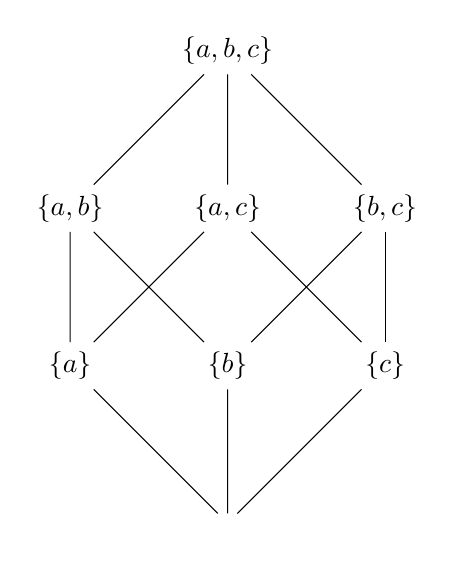
\begin{tikzpicture}[scale=2]
      \node (0) at (1,0) {$\varnothing$};
      \node (a) at (0,1) {$\{a\}$};
      \node (b) at (1,1) {$\{b\}$};
      \node (c) at (2,1) {$\{c\}$};
      \node (ab) at (0,2) {$\{a,b\}$};
      \node (ac) at (1,2) {$\{a,c\}$};
      \node (bc) at (2,2) {$\{b,c\}$};
      \node (abc) at (1,3) {$\{a,b,c\}$};
      \draw (0) -- (a) -- (ab) -- (abc) -- (ac) -- (c) -- (0);
      \draw (0) -- (b) -- (bc) -- (abc);
      \draw (a) -- (ac);
      \draw (b) -- (ab);
      \draw (c) -- (bc);
    \end{tikzpicture}
    \end{center}
    \end{bsp}


    \begin{ueb}
    Das Hasse-Diagramm einer Halbordnung auf der Menge $\{0,\dots,7 \}$ ist wie folgt gegeben.
    \begin{center}
    \begin{tikzpicture}[scale=1.5]
      \node (0) at (1,0) {$0$};
      \node (1) at (0,0) {$1$};
      \node (2) at (1,1) {$2$};
      \node (3) at (2,1) {$3$};
      \node (4) at (0,2) {$4$};
      \node (5) at (1,2) {$5$};
      \node (6) at (2,2) {$6$};
      \node (7) at (1,3) {$7$};
      \draw (0) -- (2) -- (5) -- (7) -- (6) -- (3);
      \draw (2) -- (4) ;
      \draw (1) -- (2);
    \end{tikzpicture}
    \end{center}
    \begin{enumerate}
    \item Geben Sie alle maximalen und alle minimalen Elemente von der Menge $\{0,\dots,7\}$ an.
    \item Geben Sie drei paarweise unvergleichbare Elemente an.
    \end{enumerate}
    \end{ueb}

    \begin{lsg}~
        \ifthenelse{\boolean{ml}}{~
            \begin{itemize}
                \item Minimale Elemente: $ 0,1,3$
                \item Maximale Elemente: $4,7$
                \item Drei paarweise unvergleichbare Elemente: Z.B. $1,0,3$ oder $4,5,6$ usw.
            \end{itemize}
            }{~
            \answerspace{6cm}}
    \end{lsg}


    \begin{ueb}
    Der Graph $G=(\{12,13,14,18,112 \},\preceq)$ ist wie folgt gegeben.
    \begin{center}
    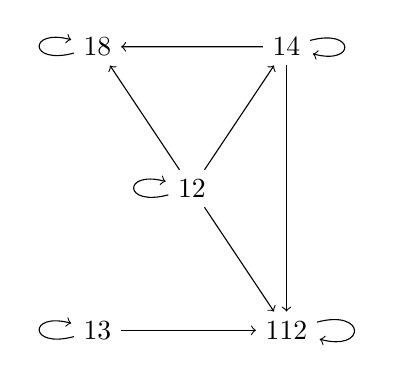
\begin{tikzpicture}[scale=1.2]
      \node (2) at (0,1.5) {$12$};
      \node (3) at (-1,0) {$13$};
      \node (4) at (1,3) {$14$};
      \node (8) at (-1,3) {$18$};
      \node (12) at (1,0) {$112$};
      \path[->] (2) edge (4) edge (8) edge (12) edge [loop left] (2);
      \path[->] (3) edge (12) edge [loop left] (3);
      \path[->] (4) edge (12) edge (8) edge [loop right] (4);
      \path[->] (8) edge [loop left] (8);
      \path[->] (12) edge [loop right] (12);
    \end{tikzpicture}
    \end{center}
    \begin{enumerate}
    \item Zeichnen Sie ein Hasse-Diagramm für die Halbordnung $\preceq$.
    \item Geben Sie die Relation als Menge an.
    \end{enumerate}
    \end{ueb}
    \begin{lsg}
        \ifthenelse{\boolean{ml}}{
            \begin{enumerate}~
                \item~
                    \begin{center}
                        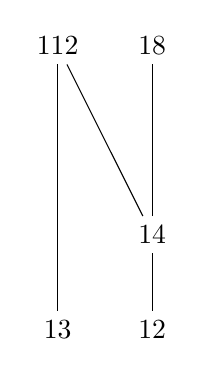
\begin{tikzpicture}[scale=1.2]
                        \node (2) at (0,0) {$12$};
                        \node (3) at (-1,0) {$13$};
                        \node (4) at (0,1) {$14$};
                        \node (8) at (0,3) {$18$};
                        \node (12) at (-1,3) {$112$};
                        \path[-] (2) edge (4);
                        \path[-] (3) edge (12);
                        \path[-] (4) edge (8);
                        \path[-] (4) edge (12);
                        \end{tikzpicture}
                    \end{center}
                \item $\{(13,13),(13,112),(12,12),(12,112),(12,14),(12,18),(14,14),(14,112),$ $(14,18),(18,18),(112,112) \}$
            \end{enumerate}
            }{~
            \answerspace{6cm}}
\end{lsg}